\chapter{Concurrency}
To understand concurrency, we must first distinguish between the abstract idea of an algorithm and its physical realization. A \textit{sequential algorithm}\index{sequential algorithm} serves as the "idea"—it is a formal description of the behavior of an abstract sequential state machine, detailing the transitions that must be executed in order. When this algorithm is translated into a specific programming language, it becomes a program, or the "text". The \textit{process}\index{process} represents the "action"; it is the dynamic entity generated when a program is executed on a concrete machine. At any given moment, a process is defined by its state, which includes its program counter and register values. A sequential process, often referred to as a thread, is managed by a single control flow and program counter.

\textit{Concurrency}\index{concurrency} arises when a set of these sequential state machines run simultaneously and interact through a communication medium, such as shared memory. This creates a multiprocess program or concurrent system. There are significant advantages to this approach: it allows for the combination of work from different processes to solve distinct tasks in parallel, and it simplifies complex programming tasks by breaking them down into more manageable, simpler components.

\section{Features of a Concurrent System}
Concurrent systems can be categorized by several key assumptions regarding their reliability and timing. In our study, we focus on systems that are reliable, asynchronous, and utilize shared memory.
\begin{itemize}
    \item \textit{Reliability:}\index{reliability} Every process is assumed to be reliable, meaning it correctly executes the code of its corresponding algorithm.
    \item \textit{Asynchrony:}\index{asynchrony} An asynchronous system makes no timing assumptions. Each process operates on its own independent clock and proceeds at an arbitrary speed.
    \item \textit{Shared Memory:}\index{shared memory} While every process has its own local memory accessible only to itself, the system includes shared registers or memory locations that can be accessed by every process in the program.
\end{itemize}
    
Regarding hardware, we often simplify the model by assuming there is one processor available for every process, allowing them to execute in parallel. However, in systems where there are fewer processors than processes, a hidden scheduler is responsible for assigning processors to processes.

\section{Process Synchronization: Cooperation and Competition}
\textit{Synchronization}\index{synchronization} occurs whenever the progress of one process depends on the behavior of others. These interactions generally fall into two categories: cooperation and competition.

\subsection{Cooperation}
In \textit{cooperation}\index{cooperation}, different processes work together to ensure they all succeed in their respective tasks.
\begin{itemize}
    \item \textit{Rendezvous (Barrier):}\index{rendezvous} A synchronization barrier is a set of control points, one for each process involved. A process is only permitted to pass its control point once every other involved process has reached its own. This forces processes to stop and wait for one another, ensuring they are synchronized at a specific stage of execution.
    \item \textit{Producer-Consumer:}\index{producer-consumer} This common pattern involves two types of processes: the producer, which generates data items, and the consumer, which utilizes them. This cooperation is governed by two strict constraints: only data that has been produced can be consumed, and every item produced must be consumed exactly once.
\end{itemize}

\subsection{Competition}
\textit{Competition}\index{competition} occurs when multiple processes attempt to execute specific actions or access a shared resource, but only one (or a limited number) can succeed at a time. A classic example is two processes attempting to withdraw 1M€ from the same bank account simultaneously.

\begin{lstlisting}[mathescape, caption={Withdraw from account balance.}, captionpos=b]
function withdraw() {
    x := account.read();
    if x $\geq$ 1M$€$ then account.write(x - 1M$€$)
}
\end{lstlisting}

Consider the \texttt{withdraw()} function that reads the account balance, checks if it is at least 1M€, and then writes the new balance. While individual read and write operations are typically atomic to happen instantaneously at a single point in time—their sequential composition within the function is not.

\begin{figure}[ht]
    \centering
    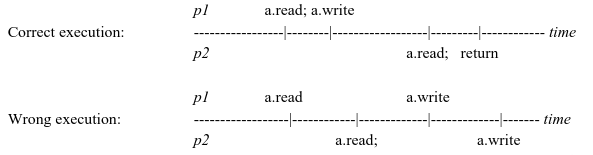
\includegraphics[width=0.7\linewidth]{images/withdraw-executions.png}
    \caption{Process executions of \texttt{withdraw()} function.}
    \label{fig:withdraw-executions}
\end{figure}

In a correct execution, process $p_1$ might complete its read and write before $p_2$ begins. However, in a wrong execution caused by interleaving, both $p_1$ and $p_2$ might read the account balance while it is still 1M€. Both will see the condition as true and proceed to write a new balance of 0€, effectively withdrawing 2M€ from an account that only contained 1M€.

\chapter{Mutual Exclusion (MUTEX)}
To resolve the issues presented by competition, we use \textit{Mutual Exclusion}\index{mutual exclusion}, which ensures that specific parts of code are executed as if they were atomic, without intermission from other processes. This is necessary not only for competition but also for cooperation when accessing shared resources.

A \textit{Critical Section}\index{critical section} (C.S.) is a part of the code that must be executed by at most one process at a time. The Mutual Exclusion problem involves designing an entry protocol (often called \texttt{lock}) and an exit protocol (\texttt{unlock}) to encapsulate the critical section.

We operate under two main assumptions:
\begin{enumerate}
    \item All critical sections will eventually terminate if executed by a single process.
    \item The code is well-formed, meaning processes always follow the sequence of locking, executing the critical section, and then unlocking.
\end{enumerate}

\section{Safety and Liveness Properties}
The effectiveness of any synchronization solution is judged by two types of properties: Safety and Liveness.
\begin{itemize}
    \item \textit{Safety:}\index{safety} "Nothing bad ever happens." In the context of MUTEX, the safety property is mutual exclusion itself: at most one process is in the critical section at any given time.
    \item \textit{Liveness:}\index{liveness} "Something good eventually happens." Liveness ensures the system remains meaningful; for instance, a system that simply forbids all activity would be safe but useless because no process would ever enter the critical section.
\end{itemize}

For Mutual Exclusion, there are three main tiers of liveness:
\begin{enumerate}
    \item \textit{Deadlock-freedom:}\index{deadlock-freedom} This is the weakest liveness property. It states that if one or more processes are trying to enter the critical section, eventually at least one of them will succeed. It focuses on system-wide progress rather than individual process progress.
    \item \textit{Starvation-freedom:}\index{starvation-freedom} A stronger property ensuring that every process that attempts to enter the critical section will eventually be granted access. This is more meaningful from the perspective of an individual "client" process.
    \item \textit{Bounded bypass:}\index{bounded bypass} The strongest property, stating that there is a limit—defined by a function $f(n)$—to how many times a process can be "bypassed" by others before it is granted entry to the critical section.
\end{enumerate}

These properties form a strict hierarchy where 
\begin{equation*}
    \text{Bounded bypass} \implies \text{Starvation-freedom} \implies \text{Deadlock-freedom}.
\end{equation*}

\begin{figure}[ht]
    \centering
    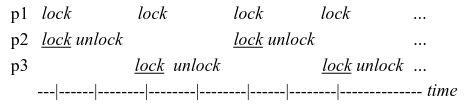
\includegraphics[width=0.6\linewidth]{images/hierarchy-of-liveness-properties.png}
    \caption{Hierarchy of liveness properties process executions (underlined actions succeed).}
    \label{fig:hierarchy-of-liveness-properties}
\end{figure}

The inclusions are strict, meaning the reverse is not necessarily true. For example, Deadlock-freedom does not imply Starvation-freedom. Consider three processes ($p_1$,$p_2$,$p_3$) repeatedly trying to enter a critical section. It is possible for $p_2$ and $p_3$ to alternate winning the competition, continually bypassing $p_1$. In this scenario, the system is deadlock-free because progress is being made ($p_2$ and $p_3$ are entering the C.S.), but it is not starvation-free because $p_1$ is locked out forever.

Similarly, Starvation-freedom does not imply Bounded bypass. While starvation-freedom guarantees that a process will eventually enter (the number of bypasses is finite), it does not provide a specific mathematical bound ($f(n)$) on how many times that process might be overtaken before its turn arrives.

\section{Atomic Read/Write Registers}
In the study of concurrent systems, the complexity and correctness of an algorithm often depend on the level of atomicity provided by the underlying hardware. We begin by considering Atomic Read/Write (R/W) registers. These are basic storage units that support two fundamental operations: \texttt{READ} and \texttt{WRITE}. For a register to be considered "atomic," it must satisfy specific properties that allow us to reason about it as if operations occur instantaneously.

An atomic register ensures that every operation invocation behaves as though it takes place at a single, distinct point on a timeline. Formally, there exists a function $t$ that maps each operation invocation to a positive real number. This point $t$ must fall within the actual time interval of the operation—between its start and its end. Furthermore, this function is injective, meaning that two operations cannot happen at the same logical moment. From a data consistency perspective, an atomic register guarantees that any \texttt{READ} operation returns the value written by the most recent \texttt{WRITE} that preceded it, or the initial value if no \texttt{WRITE} has yet occurred.

These registers are further classified by their accessibility. A Single-Read/Single-Write (SRSW) register is the most restrictive, allowing only one specific process to read and one specific process to write. As we scale, we encounter Single-Read/Multiple-Write (SRMW), Multiple-Read/Single-Write (MRSW), and finally, Multiple-Read/Multiple-Write (MRMW) registers, which allow any process to perform the designated operations.

\section{The Peterson Algorithm}
The \textit{Peterson algorithm}\index{Peterson algorithm} is a classic solution to the mutual exclusion (MUTEX) problem. To understand its final form, we can examine the failures of simpler attempts to coordinate two processes, $p_0$ and $p_1$.

In a first attempt, we might use a single shared variable, \texttt{LAST}, to act as an indicator. When a process $i$ wants to enter the critical section, it sets \texttt{LAST} to its own ID and waits until \texttt{LAST} is no longer equal to $i$. 

\begin{minipage}{\textwidth}
\begin{minipage}{0.45\textwidth}
\begin{lstlisting}[mathescape]
lock(i) :=
    LAST $\leftarrow$ i
    wait LAST $\neq$ i
    return
\end{lstlisting}
\end{minipage}
\hfill
\begin{minipage}{0.45\textwidth}
\begin{lstlisting}[mathescape]
unlock(i) :=
    return
\end{lstlisting}
\end{minipage}
\captionof{lstlisting}{Wrong Peterson algorithm.}
\end{minipage}\\

While this ensures that two processes cannot both enter the critical section (since the variable can only hold one value), it suffers from liveness flaw: if only one process ever tries to lock, it will set the variable to its own ID and wait forever for a second process that never arrives to change it.

In a second attempt, we might use a \texttt{FLAG} array where \texttt{FLAG[i]} indicates process i's intent to enter the critical section. A process sets its flag to "up" and waits for the other process's flag to be "down." 

\begin{minipage}{\textwidth}
\begin{lstlisting}[mathescape]
Initialize FLAG[0] and FLAG[1] to down
\end{lstlisting}
\begin{minipage}{0.45\textwidth}
\begin{lstlisting}[mathescape]
lock(i) :=
    FLAG[i] $\leftarrow$ up
    wait FLAG[1-i] = down
    return
\end{lstlisting}
\end{minipage}
\hfill
\begin{minipage}{0.45\textwidth}
\begin{lstlisting}[mathescape]
unlock(i) :=
    FLAG[i] $\leftarrow$ down
    return
\end{lstlisting}
\end{minipage}
\captionof{lstlisting}{Wrong Peterson algorithm.}
\end{minipage}\\

This approach also fails due to deadlock. If both processes simultaneously raise their flags, they will both enter the wait state, each waiting for the other to lower their flag, which will never happen.

The correct Peterson algorithm combines these two ideas: the \texttt{FLAG} array to indicate intent and the \texttt{LAST} variable to break ties.

\begin{minipage}{\textwidth}
\begin{lstlisting}[mathescape]
Initialize FLAG[0] and FLAG[1] to down
\end{lstlisting}
\begin{minipage}{0.45\textwidth}
\begin{lstlisting}[mathescape]
lock(i) :=
    FLAG[i] $\leftarrow$ up
    LAST $\leftarrow$ i
    wait (FLAG[1-i] = down 
        OR LAST $\neq$ i)
    return
\end{lstlisting}
\end{minipage}
\hfill
\begin{minipage}{0.45\textwidth}
\begin{lstlisting}[mathescape]
unlock(i) :=
    FLAG[i] $\leftarrow$ down
    return
\end{lstlisting}
\end{minipage}
\captionof{lstlisting}{Correct solution to the Peterson algorithm.}
\end{minipage}\\

In this protocol, a process $p_i$ first signals its intent by raising its flag. Crucially, it then sets \texttt{LAST} to its own index, essentially saying "I am interested, but the other process can go first if it wants to." It only enters the critical section if either the other process is uninterested (its flag is down) or the other process have setting \texttt{LAST} to its own index.\\

\begin{Demonstration}{MUTEX proof for Peterson algorithm}{}
To prove that Peterson's algorithm satisfies MUTEX, we can use a proof by contradiction. Assume that both $p_0$ and $p_1$ are in the critical section simultaneously. For $p_0$ to have entered, its wait condition must have been false. This could happen in two scenarios:
\begin{enumerate}
    \item \texttt{FLAG[1]} was down: This implies that when $p_0$ checked the flag, $p_1$ had not yet raised its flag or had already exited. However, for $p_1$ to be in the critical section, it must have eventually raised its flag and set \texttt{LAST} to 1. If $p_1$ raised its flag after $p_0$ checked it, $p_1$ would then set \texttt{LAST} to 1 and find $p_0$'s flag already up, causing $p_1$ to wait.
    
    \begin{minipage}{\textwidth}
        \centering
        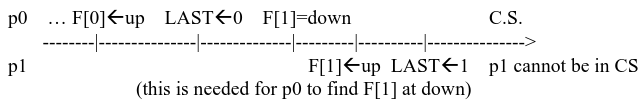
\includegraphics[width=0.7\linewidth]{images/mutex-proof-peterson1.png}
        \captionof{figure}{First case of the MUTEX proof for Peterson Algorithm.}
    \end{minipage}
    
    \item \texttt{LAST} was 1: For $p_0$ to see \texttt{LAST} as 1 (not 0), $p_1$ must have been the last one to write to that variable. If $p_1$ was the last to write, then $p_1$ would find \texttt{LAST == 1} and \texttt{FLAG[0] == up}, forcing $p_1$ to wait.
    
    \begin{minipage}{\textwidth}
        \centering
        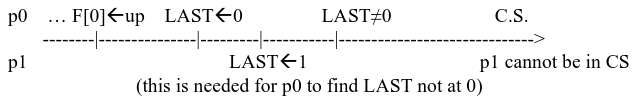
\includegraphics[width=0.7\linewidth]{images/mutex-proof-peterson2.png}
        \captionof{figure}{Second case of the MUTEX proof for Peterson Algorithm.}
    \end{minipage}
\end{enumerate}
In both cases, it is impossible for both processes to pass the wait condition at the same time.
\end{Demonstration}

\begin{Demonstration}{Bounded Bypass proof for Peterson algorithm}{}
Peterson's algorithm for two processes provides a bounded bypass of 1. This means that if $p_0$ is waiting to enter, $p_1$ can enter and exit the critical section at most once before $p_0$ is guaranteed entry.

If $p_0$ is blocked, it means \texttt{FLAG[1]} is "up" and \texttt{LAST} is 0. This implies $p_1$ is either in the critical section or about to enter. When $p_1$ exits, it sets \texttt{FLAG[1]} to "down." If $p_1$ tries to re-enter immediately, it must set \texttt{LAST} to 1. At that point, $p_0$ will see that \texttt{LAST} is no longer 0 and will be able to enter the critical section.
\end{Demonstration}

\subsection{Peterson's Algorithm for $n$ Processes}
The algorithm can be generalized to $n$ processes by visualizing it as a series of $n-1$ levels. A process must pass through each level—like a filter—to reach the critical section. At each level, at least one process is "left behind," effectively reducing the number of processes that can proceed to the next level.

The \texttt{FLAG} array now tracks which level a process has reached, and an array of \texttt{LAST} variables (one for each level) acts as the tie-breaker for that specific level.

\begin{minipage}{\textwidth}
\begin{lstlisting}[mathescape]
Initialize FLAG[i] to 0, for all i
\end{lstlisting}
\begin{minipage}{0.45\textwidth}
\begin{lstlisting}[mathescape]
lock(i) :=
    for lev = 1 to n-1 do
        FLAG[i] $\leftarrow$ lev
        LAST[lev] $\leftarrow$ i
        wait ($\forall$k$\neq$i FLAG[k] < lev
            OR LAST[lev] $\neq$ i)
    return
\end{lstlisting}
\end{minipage}
\hfill
\begin{minipage}{0.45\textwidth}
\begin{lstlisting}[mathescape]
unlock(i) :=
    FLAG[i] $\leftarrow$ 0
    return
\end{lstlisting}
\end{minipage}
\captionof{lstlisting}{Peterson algorithm for $n$ processes.}
\end{minipage}\\

\begin{Lemma}{MUTEX proof for Peterson algorithm for $n$ processes}{}
The safety of the $n$-process algorithm rests on the lemma that for every level $\ell\in\{0,\ldots,n-1\}$, at most $n-\ell$ processes can be at that level. By the time we reach level $n-1$, only $(n-(n-1))=1$ process can remain, satisfying MUTEX.
\begin{demonstration}
This is proven by induction on $\ell$. The base case $(\ell=0)$ is trivial, as all $n$ processes start at level 0. For the inductive step, we consider the last process $p_x$ to write to \texttt{LAST}[$\ell$+1]. For $p_x$ to pass to level $\ell+1$, all other processes $p_k$ must have a flag value lower than $\ell+1$. If $p_x$ is blocked, and since at most $n-\ell$ processes reached level $\ell$, there are at most $n-\ell-1$ processes that can potentially be at level $\ell+1$ while $p_x$ waits.
\end{demonstration}
\end{Lemma}

\begin{Lemma}{Starvation freedom proof for Peterson algorithm for $n$ processes}{}
The algorithm is starvation-free, meaning every process at level $\ell$ eventually reaches level $\ell+1$ and, ultimately, the critical section. 
\begin{demonstration}
This is proven by reverse induction from level $n-1$ down to 0. If a process $p_x$ is blocked at level $\ell$, it must be that \texttt{LAST}[$\ell$+1] == x and some other process $p_y$ has a flag value $\geq\ell+1$. By the inductive hypothesis, $p_y$ will eventually progress and exit. If no other process enters level $\ell+1$ to change the \texttt{LAST} variable, $p_x$ will eventually be the only process at that level and will pass the wait condition.
\end{demonstration}
\end{Lemma}

The $n$-process Peterson algorithm is robust but comes with specific memory and performance costs. It requires $n$ MRSW registers for the \texttt{FLAG} array and $n-1$ MRMW registers for the \texttt{LAST} array. Each entry into the critical section requires $(n-1)\times(n+2)$ register accesses for locking and 1 access for unlocking.

While it guarantees starvation freedom, the $n$-process version does not satisfy bounded bypass. Because a process can "sleep" arbitrarily long during its first wait, other processes can theoretically enter and exit the critical section an unbounded number of times before the sleeping process wakes up and progresses to the next level.

Finally, the algorithm is easily generalized to $k$-MUTEX, where up to $k$ processes are allowed in the critical section simultaneously. This is achieved by simply reducing the number of levels in the loop from $n-1$ to $n-k$.

\section{Concurrent Algorithms With Better Performance}
Peterson’s algorithm, while effective for two processes, becomes computationally expensive when generalized to $n$ processes. In its standard $n$-process form, it requires a process to compete across $n-1$ levels, leading to a contention-free time complexity of $O(n^2)$. To optimize this, we can employ a tournament-based approach.

This approach utilizes a complete binary tree where each node represents a 2-process mutual exclusion algorithm (such as Peterson’s). For $n$ processes, the tree has a height of $\lceil\log_2{n}\rceil$. A process wishing to enter the Critical Section (CS) must "win" a competition at each level of the tree, starting from a leaf and moving toward the root. Since each competition at a node has a constant cost, the total cost to reach the CS is reduced to $O(\log{n})$.

\begin{figure}[ht]
    \centering
    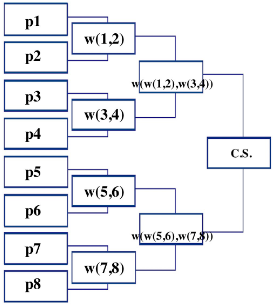
\includegraphics[width=0.4\linewidth]{images/tournament-based-tree.png}
    \caption{Tournament-based algorithm tree.}
    \label{fig:tournament-based-tree}
\end{figure}

The quest for even greater efficiency leads to the exploration of $O(1)$ algorithms. Ideally, in a "contention-free" scenario (where only one process is active), the process should be able to enter its CS with a fixed, small number of register accesses.

The initial idea for such an algorithm involves two shared registers: \texttt{X} and \texttt{Y}. \texttt{X} is used to track the identity of the process currently attempting to lock, while \texttt{Y} acts as a "gatekeeper." 

\begin{minipage}{\textwidth}
\begin{lstlisting}[mathescape]
Initialize Y at $\perp$, X at any value (e.g., 0)
\end{lstlisting}
\begin{minipage}{0.45\textwidth}
\begin{lstlisting}[mathescape]
lock(i) :=
    X $\leftarrow$ i
    if Y $\neq$ $\perp$ then FAIL
        else Y $\leftarrow$ i
            if X = i then return
                else FAIL
\end{lstlisting}
\end{minipage}
\hfill
\begin{minipage}{0.45\textwidth}
\begin{lstlisting}[mathescape]
unlock(i) :=
    Y $\leftarrow$ $\perp$
    return
\end{lstlisting}
\end{minipage}
\captionof{lstlisting}{Constant-time algorithm for $n$ processes.}
\end{minipage}\\

In a simplified version, a process $i$ writes its ID to \texttt{X} and then checks \texttt{Y}. If \texttt{Y} is already set, the process \texttt{FAIL}. Otherwise, it sets \texttt{Y} to $i$ and checks if \texttt{X} is still equal to $i$. If both conditions hold, the process enters the CS. Without contention, this requires only four register accesses.

However, this \texttt{FAIL} mechanism is problematic because it forces processes to repeatedly retry the lock, which can lead to a deadlock. Specifically, a scenario can occur where multiple processes interfere with each other's \texttt{X} and \texttt{Y} values such that no process ever successfully enters the CS.

\subsection{Lamport’s Fast MUTEX Algorithm}
To resolve the deadlock issue while maintaining $O(1)$ complexity in the absence of contention, Leslie Lamport designed the Fast Mutex Algorithm. This algorithm uses an array of flags (\texttt{FLAG[1..n]}) and two shared registers, \texttt{X} and \texttt{Y} (with \texttt{Y} initialized to $\perp$).

\begin{minipage}{\textwidth}
\begin{lstlisting}[mathescape]
Initialize Y at $\perp$, X at any value (e.g., 0)
\end{lstlisting}
\begin{lstlisting}[mathescape]
lock(i) :=
*   FLAG[i] $\leftarrow$ up
    X $\leftarrow$ i
    if Y $\neq$ $\perp$ then FLAG[i] $\leftarrow$ down
                   wait Y = $\perp$
                   goto *
        else Y $\leftarrow$ i
            if X = i then return
                else FLAG[i] $\leftarrow$ down
                    $\forall$ j wait FLAG[j] = down
                    if Y = i then return
                        else wait Y = $\perp$
                             goto *
\end{lstlisting}
\begin{lstlisting}[mathescape]
unlock(i) :=
    Y $\leftarrow$ $\perp$
    FLAG[i] $\leftarrow$ down
    return
\end{lstlisting}
\captionof{lstlisting}{Lamport’s Fast MUTEX Algorithm.}
\end{minipage}\\

The logic for \texttt{lock(i)} is as follows:
\begin{enumerate}
    \item Process $p_i$ sets \texttt{FLAG[i]} to up and writes its identity to \texttt{X}.
    \item It checks \texttt{Y}. If \texttt{Y}$\neq\perp$, it knows another process is active. It resets its flag to down, waits for \texttt{Y} to become $\perp$, and then restarts the protocol.
    \item If \texttt{Y}$=\perp$, it sets \texttt{Y} to $i$. It then checks if \texttt{X} is still $i$. If \texttt{X}$=i$, the process has secured the "fast path" and enters the CS immediately. This takes only five accesses in contention-free scenarios.
    \item If X$\neq i$ (meaning someone else overwrote \texttt{X}), the process must take the "slow path." It resets its flag, waits for all other processes to lower their flags, and then performs a final check on \texttt{Y}. If \texttt{Y} is still $i$, it enters the CS; otherwise, it waits for \texttt{Y} to be cleared and restarts.
\end{enumerate}

The \texttt{unlock(i)} procedure is simple: $p_i$ resets \texttt{Y} to $\perp$ and then lowers its \texttt{FLAG[i]}.

\begin{Demonstration}{MUTEX proof for Lamport’s Fast MUTEX Algorithm}{}
Mutual exclusion ensures that if process $p_i$ is in the CS, no other process $p_j$ can be there simultaneously. The proof considers the two ways $p_i$ can enter the CS:
\begin{itemize}
    \item If $p_i$ enters because it read \texttt{X = i}, it must have written \texttt{Y = i} after checking that \texttt{Y} was $\perp$. For $p_j$ to enter, it would also need to find \texttt{Y} at $\perp$. If $p_j$ wrote to \texttt{X} after $p_i$ did, $p_i$ would not have read \texttt{X = i}. Therefore, $p_j$ must have written \texttt{X} earlier. However, this means $p_j$ will find \texttt{Y = i} (set by $p_i$) and be forced to wait for $p_i$ to unlock.
    
    \begin{minipage}{\textwidth}
        \centering
        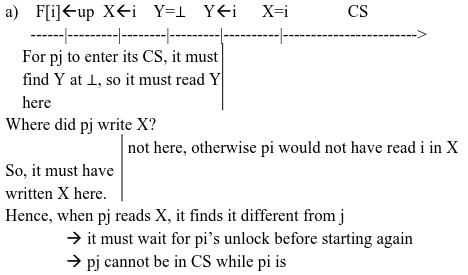
\includegraphics[width=0.5\linewidth]{images/lamport-mutex-proof1.png}
        \captionof{figure}{First case of the MUTEX proof for Lamport’s Fast MUTEX Algorithm.}
    \end{minipage}
    
    \item If $p_i$ enters via the slow path, it must have waited until all \texttt{FLAG[k]} were down. If $p_j$ tries to enter, it must either finish its CS before $p_i$ starts or be blocked by the fact that $p_i$ has set \texttt{Y}$=i$. Since $p_i$ only resets \texttt{Y} upon unlocking, $p_j$ cannot progress past the gatekeeper check until $p_i$ is finished.
    
    \begin{minipage}{\textwidth}
        \centering
        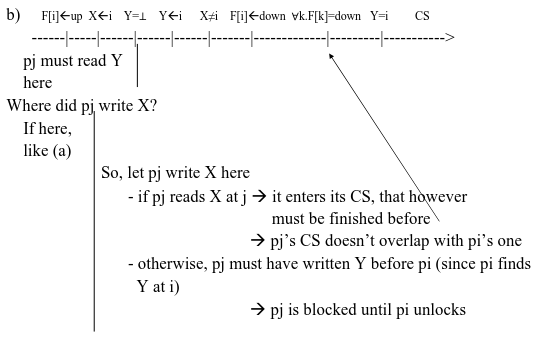
\includegraphics[width=0.65\linewidth]{images/lamport-mutex-proof2.png}
        \captionof{figure}{Second case of the MUTEX proof for Lamport’s Fast MUTEX Algorithm.}
    \end{minipage}
    
\end{itemize}
\end{Demonstration}

\begin{Demonstration}{Deadlock freedom proof for Lamport’s Fast MUTEX Algorithm}{}
Deadlock freedom ensures that if a process invokes lock, at least one process eventually enters the CS. The proof analyzes the three points where a process might be blocked:
\begin{enumerate}
    \item Second wait \texttt{Y}$= \perp$: If $p_i$ is blocked here, it means it read a value in \texttt{Y} other than $i$. This implies another process $p_h$ wrote to \texttt{Y} after $p_i$. By considering the "last" such process to write to \texttt{Y}, that process is guaranteed to eventually enter the CS or clear the way.
    \item $\forall j$ \texttt{wait FLAG[j] = down}: This wait cannot block a process forever. If $p_j$ is not trying to lock, its flag is down. If $p_j$ is trying to lock but fails the \texttt{Y} or \texttt{X} checks, it eventually sets its flag to down. If $p_j$ enters the CS, it will eventually unlock and set the flag to down.
    \item First wait \texttt{Y} $= \perp$: If $p_i$ is stuck here, it means some $p_k$ wrote to \texttt{Y} first. As shown in the previous points, $p_k$ will either enter the CS and eventually unlock (clearing \texttt{Y}) or it will be blocked elsewhere in a way that allows progress.
\end{enumerate}
\end{Demonstration}

With atomic read/write registers, the trade-offs between different algorithms for $n$ processes are summarized below in Table \ref{tab:summary-complexity}.
\begin{table}[ht]
    \centering
    \begin{tabular}{|l|p{3.1cm}|l|}
         \hline
         \textbf{Algorithm Type} & \textbf{Complexity (Contention-Free)} & \textbf{Liveness Property}\\
         \hline
         Peterson (standard) & $O(n^2)$ & Starvation-Freedom\\
         \hline
         Tournament-based & $O(\log n)$ & Bounded Bypass\\
         \hline
         Lamport Fast MUTEX & $O(1)$ & Deadlock-Freedom\\
         \hline
    \end{tabular}
    \caption{Summary of complexity for concurrent algorithms.}
    \label{tab:summary-complexity}
\end{table}

While Lamport's algorithm provides O(1) complexity and deadlock freedom, it is important to note that it can lead to starvation, where a specific process is bypassed indefinitely even though the system as a whole is making progress. Every deadlock-free algorithm can be transformed into a bounded bypass one, but this often comes at the cost of increased complexity.

\section{Turn Deadlock Freedom into Bounded Bypass}
To understand the progression of mutual exclusion algorithms, we must examine how a protocol that guarantees only basic deadlock freedom can be elevated to provide a stronger progress condition: bounded bypass.
The goal of this transformation is to take any deadlock-free protocol (denoted here as DLF) and wrap it in a structure that enforces fairness. This is achieved through the Round Robin algorithm. The name "Round Robin" itself finds its origins in the medieval French custom of signing petitions in a circular fashion—Ruban Rond or "round ribbon"—to obscure the identity of the leader or initiator, ensuring all participants shared equal standing. In the context of concurrent systems, it implies a circular, fair distribution of access.

The algorithm utilizes an array of flags, \texttt{FLAG[i]}, initialized to down for all processes, and a shared register \texttt{TURN}, which can be initialized to any process \texttt{ID}. 

\begin{minipage}{\textwidth}
\begin{lstlisting}[mathescape]
Initialize FLAG[i] to down ($\forall$ i) and TURN to any proc.id.
\end{lstlisting}
\begin{minipage}{0.45\textwidth}
\begin{lstlisting}[mathescape]
lock(i) :=
    FLAG[i] $\leftarrow$ up
    wait (TURN = i OR
          FLAG[TURN] = down)
    DLF.lock(i)
    return
\end{lstlisting}
\end{minipage}
\hfill
\begin{minipage}{0.45\textwidth}
\begin{lstlisting}[mathescape]
unlock(i) :=
    FLAG[i] $\leftarrow$ down
    if FLAG[TURN] = down then
        TURN $\leftarrow$ (TURN+1) mod n
    DLF.unlock(i)
    return
\end{lstlisting}
\end{minipage}
\captionof{lstlisting}{Round Robin algorithm to turn a deadlock free protocol into a bounded bypass protocol for MUTEX.}
\end{minipage}\\

For the entry protocol \texttt{lock(i)}, the process $p_i$ first signals its intent by setting \texttt{FLAG[i]} to up. It then enters a busy-wait period where it stays suspended until one of two conditions is met: either it is its turn or the process whose turn it currently is is not interested in the critical section. Only after passing this "gate" does the process invoke the underlying deadlock-free locking mechanism.

The exit protocol \texttt{unlock(i)} mirrors this structure. The process first releases the underlying lock via \texttt{DLF.unlock(i)}. Then, it lowers its own flag and, if the current turn belongs to it, it increments the \texttt{TURN} variable to the next process in a circular fashion using the modulo operator.

The proof of deadlock freedom for the Round Robin algorithm relies on the fact that if at least one process invokes \texttt{RR.lock}, at least one process will eventually enter the critical section. Since we know the underlying DLF is deadlock-free, we simply need to prove that at least one process will eventually exit the initial wait statement to invoke \texttt{DLF.lock}.

If we assume \texttt{TURN=k}, and process $p_k$ has invoked the lock, it will find that \texttt{TURN = k} is true and immediately proceed to \texttt{DLF.lock}. If $p_k$ has not invoked the lock, its \texttt{FLAG[k]} will be down. In this case, any other process $p_i$ that has invoked the lock will find that \texttt{FLAG[TURN] = down} is true and will likewise proceed to the underlying lock. Thus, the system as a whole cannot get stuck at the wrapper level.

To prove the bounded bypass property, we must quantify how long a process might have to wait.

\begin{Lemma}{Bounded bypass proof for Round Robin algorithm for MUTEX}{}\label{lemma:bounded-bypass-RR1}
If it is currently $p_i$'s turn (\texttt{TURN = i}) and $p_i$ is interested (\texttt{FLAG[i] = up}), it will enter the critical section in at most $(n-1)$ iterations of other processes.

\begin{demonstration}
This is supported by three key observations. First, \texttt{TURN} only changes when the process currently holding the turn sets its flag to down, which only happens after it finishes its critical section. Second, if $p_i$ has its flag up, it is either already in the critical section or is currently competing within the \texttt{DLF.lock} primitive. Third, any process $p_j$ that invokes the lock after $p_i$ has already set its flag will be blocked at the initial wait statement because \texttt{TURN = i} and \texttt{FLAG[i] = up}.

Consequently, we can define a set \texttt{Y} of processes currently competing for the critical section (those suspended on \texttt{DLF.lock}). Once $p_i$ sets its flag, this set \texttt{Y} cannot grow. Because the underlying DLF is deadlock-free, some process $p_y$ in \texttt{Y} must eventually win. If that process is $p_i$, the lemma is satisfied. If it is another process, that process enters the critical section, exits, and because \texttt{TURN} remains $i$, that process cannot re-enter the set \texttt{Y}. Thus, \texttt{Y} shrinks by one with each winner until $p_i$ is eventually the only one left to win. The worst-case scenario is when \texttt{Y} contains all $n$ processes, requiring $n-1$ other processes to finish before $p_i$.
\end{demonstration}
\end{Lemma}

\begin{Lemma}{Bounded bypass proof for Round Robin algorithm for MUTEX}{}\label{lemma:bounded-bypass-RR2}
If $p_i$ is interested, \texttt{TURN} will be set to $i$ in at most $(n-1)^2$ iterations. 

\begin{demonstration}
If \texttt{TURN} is not already $i$, we know by the deadlock freedom of the Round Robin wrapper that at least one process will eventually unlock. If the process whose turn it is ($p_{TURN}$) is idle, \texttt{TURN} increments immediately. If $p_{TURN}$ is active, we know from Lemma \ref{lemma:bounded-bypass-RR1} that it will win and eventually increment \texttt{TURN} in at most $(n-1)$ iterations. Since there are at most $(n-1)$ processes that could hold the turn before it reaches $i$, the total iterations are $(n-1)\times(n-1)=(n-1)^2$.
\end{demonstration}
\end{Lemma}

The combined logic of these lemmas allows us to establish the final bound for the algorithm. Bounded bypass guarantees that if a process $p_i$ invokes the lock, it will enter the critical section in at most $n(n-1)$ iterations.

The calculation is a summation of the two stages of waiting. First, $p_i$ sets its flag. According to Lemma \ref{lemma:bounded-bypass-RR2}, it may take up to $(n-1)^2$ iterations for the \texttt{TURN} variable to cycle around to $i$. Once \texttt{TURN} is equal to $i$, Lemma \ref{lemma:bounded-bypass-RR1} dictates that $p_i$ will enter the critical section in at most $(n-1)$ further iterations. Adding these together $(n-1)^2+(n-1)$ results in $n(n-1)$. This provides a strict upper bound on the number of times $p_i$ can be bypassed by other processes, successfully transforming a deadlock-free protocol into a bounded bypass one.

\section{Mutual Exclusion and Specialized Hardware}
\subsection{Specialized Hardware Primitives for Mutual Exclusion}
While atomic read/write registers offer a foundational computational model for concurrent systems, they are often too basic for complex synchronization needs. To strengthen this model, most modern operating systems and shared memory multiprocessors provide specialized hardware primitives. These are built-in, atomic operations implemented directly in the hardware, specifically designed to address synchronization issues more efficiently than solutions based on simple read/write operations.

The most common of these hardware primitives include:
\begin{itemize}
    \item \textit{Test\&set:}\index{test\&set} An atomic operation that reads a boolean register and writes a new value to it.
    \item \textit{Swap:}\index{swap} An atomic operation that exchanges the contents of a general register with a given value.
    \item \textit{Fetch\&add:}\index{fetch\&add} An atomic operation that reads an integer register and increases its value by a specified amount.
    \item \textit{Compare\&swap:}\index{compare\&swap} An atomic operation that compares the current value of a register with an expected "old" value; if they match, it updates the register to a "new" value and returns a boolean indicating success.
\end{itemize}

\subsubsection{Mutual Exclusion with Test\&set}
The Test\&set primitive is a fundamental tool for implementing locks. When applied to a boolean register \texttt{X}, it atomically performs two steps: it stores the current value of \texttt{X} in a temporary variable and then sets \texttt{X} to 1. The primitive then returns the original value stored in the temporary variable. Because this entire sequence is atomic, no other process can intervene between the read and the write.

\begin{minipage}{\textwidth}
\begin{lstlisting}[mathescape]
X.test&set() :=
    tmp $\leftarrow$ X
    X $\leftarrow$ 1
    return tmp
\end{lstlisting}
\captionof{lstlisting}{Test\&set.}
\end{minipage}\\

A simple mutual exclusion protocol can be established using this primitive. To acquire a lock, a process wait until \texttt{X.test\&set()} returns 0. 

\begin{minipage}{\textwidth}
\begin{lstlisting}[mathescape]
Initialize X at 0
\end{lstlisting}
\begin{minipage}{0.45\textwidth}
\begin{lstlisting}[mathescape]
lock(i) :=
    wait X.test&set() = 0
    return
\end{lstlisting}
\end{minipage}
\hfill
\begin{minipage}{0.45\textwidth}
\begin{lstlisting}[mathescape]
unlock(i) :=
    X $\leftarrow$ 0
    return
\end{lstlisting}
\end{minipage}
\captionof{lstlisting}{MUTEX with Test\&set.}
\end{minipage}\\

The first process to call this when \texttt{X=0} will receive 0 and simultaneously set \texttt{X} to 1, effectively "locking" the resource and causing subsequent calls by other processes to return 1. To unlock the resource, the process simply sets \texttt{X} back to 0.

\subsubsection{Mutual Exclusion with Swap}
The Swap primitive serves as a generalization of Test\&set. It atomically exchanges the value of a general register \texttt{X} with a provided value \texttt{v}, returning the old value of \texttt{X}. 

\begin{minipage}{\textwidth}
\begin{lstlisting}[mathescape]
X.swap(v) :=
    tmp $\leftarrow$ X
    X $\leftarrow$ v
    return tmp
\end{lstlisting}
\captionof{lstlisting}{Swap.}
\end{minipage}\\

This primitive is highly versatile because the previously discussed Test\&set protocol can be directly adapted to use it. Specifically, the operation \texttt{X.test\&set()} is functionally equivalent to \texttt{X.swap(1)}. By swapping in the value 1 and checking if the returned value was 0, a process can determine if it has successfully acquired the lock.

\subsubsection{Mutual Exclusion with Compare\&swap}
Compare\&swap takes two parameters, \texttt{old} and \texttt{new}, and checks if the shared register \texttt{X} currently holds the value \texttt{old}. If the condition \texttt{X=old} is met, \texttt{X} is updated to \texttt{new} and the operation returns \texttt{true}. Otherwise, the register remains unchanged, and the operation returns \texttt{false}.

\begin{minipage}{\textwidth}
\begin{lstlisting}[mathescape]
X.compare&swap(old, new) :=
    if X = old then X $\leftarrow$ new
                    return true
    return false
\end{lstlisting}
\captionof{lstlisting}{Compare\&swap.}
\end{minipage}\\

To implement mutual exclusion with Compare\&swap, the \texttt{lock()} operation involves waiting until \texttt{X.compare\&swap(0, 1)} returns \texttt{true}. This ensures that only the process that finds \texttt{X} at 0 can change it to 1 and proceed. The \texttt{unlock()} operation is a simple assignment of 0 to \texttt{X}. 

\begin{minipage}{\textwidth}
\begin{lstlisting}[mathescape]
Initialize X at 0
\end{lstlisting}
\begin{minipage}{0.45\textwidth}
\begin{lstlisting}[mathescape]
lock() :=
    wait X.compare&swap(0,1) = true
    return
\end{lstlisting}
\end{minipage}
\hfill
\begin{minipage}{0.45\textwidth}
\begin{lstlisting}[mathescape]
unlock(i) :=
     X $\leftarrow$ 0
    return
\end{lstlisting}
\end{minipage}
\captionof{lstlisting}{MUTEX with Compare\&swap.}
\end{minipage}\\

While Compare\&swap is powerful and can prevent many synchronization errors, protocols using only Test\&set, Swap, or Compare\&swap can suffer from starvation, where a process is indefinitely delayed because other processes keep winning the race to the lock.

\subsubsection{Mutual Exclusion with Fetch\&add}
To address the issue of starvation and promote better liveness properties, a Round Robin approach can be implemented using the Fetch\&add primitive. This primitive atomically adds a value \texttt{v} to an integer register \texttt{X} and returns the original value.

\begin{minipage}{\textwidth}
\begin{lstlisting}[mathescape]
X.fetch&add(v) :=
    tmp $\leftarrow$ X
    X $\leftarrow$ X+v
    return tmp
\end{lstlisting}
\captionof{lstlisting}{Fetch\&add.}
\end{minipage}\\

A robust mutual exclusion protocol using Fetch\&add employs a "ticket" system, similar to how customers are served in a bakery.

\begin{minipage}{\textwidth}
\begin{lstlisting}[mathescape]
Initialize TICKET and NEXT at 0
\end{lstlisting}
\begin{minipage}{0.45\textwidth}
\begin{lstlisting}[mathescape]
lock() :=
    my_tick $\leftarrow$ TICKET.fetch&add(1)
    wait my_tick = NEXT
    return
\end{lstlisting}
\end{minipage}
\hfill
\begin{minipage}{0.45\textwidth}
\begin{lstlisting}[mathescape]
unlock() :=
    NEXT $\leftarrow$ NEXT+1
    return
\end{lstlisting}
\end{minipage}
\captionof{lstlisting}{MUTEX with Fetch\&add.}
\end{minipage}\\

A process first obtains its unique ticket number by calling \texttt{my\_tick} $\leftarrow$ \texttt{TICKET.Fetch\&add(1)}. It then waits until its ticket matches the current turn.
Upon exiting the critical section, the process increments the turn counter to allow the next ticket holder to proceed.
 
This ticket-based algorithm ensures starvation-freedom and provides a bounded bypass of $n-1$. This means that once a process has its ticket, it will enter the critical section after at most all other $n-1$ processes that already had (or might concurrently obtain) their tickets have finished their turns.

\subsection{Safe Registers}
A critical question in concurrent systems is whether mutual exclusion can be enforced without hardware-level atomicity. \textit{Safe Register}\index{safe register} are the weakest type of register that remains useful for concurrency: unlike atomic registers, safe registers have much weaker guarantees:
\begin{itemize}
    \item  \textit{MRSW (Multi-Reader Single-Writer) Safe Register:}\index{MRSW (Multi-Reader Single-Writer)} If a \texttt{READ} operation does not overlap with a \texttt{WRITE} operation, it returns the value currently stored in the register. However, if a \texttt{READ} overlaps with a \texttt{WRITE}, the \texttt{READ} may return any value from the register's domain, even one that was never written.
    \item \textit{MRMW (Multi-Reader Multi-Writer) Safe Register:}\index{MRMW (Multi-Reader Multi-Writer)} This behaves like an \texttt{MRSW} safe register as long as \texttt{WRITE} operations do not overlap. If \texttt{WRITE} operations overlap, the register's contents can become arbitrary (any value in its domain), and subsequent \texttt{READ}s may return any value until a non-overlapping \texttt{WRITE} restores a known state.
\end{itemize}

\subsubsection{Lamport’s Bakery Algorithm (1974)}
The Bakery Algorithm, designed by Leslie Lamport, is the first algorithm created to solve the mutual exclusion problem using only these non-atomic, MRSW safe registers. The core idea is that every process wishing to enter the critical section receives a ticket. However, because the registers are not atomic, two processes might read the same current maximum ticket value and thus assign themselves identical tickets. To resolve these ties and create a total ordering, the algorithm uses a pair $\langle ticket,i\rangle$, where $i$ is the process ID.

A total order is defined lexicographically: $\langle x,i\rangle < \langle y,j\rangle$ if $x<y$, or if $x=y$ and $i<j$.

\begin{minipage}{\textwidth}
\begin{lstlisting}[mathescape]
Initialize FLAG[i] to down and MY_TURN[i] to 0, for all i
\end{lstlisting}
\begin{lstlisting}[mathescape]
lock(i) :=
    FLAG[i] $\leftarrow$ up
    MY_TURN[i] $\leftarrow$ max{MY_TURN[1$\ldots$,MY_TURN[n]}+1
    FLAG[i] $\leftarrow$ down
    forall j $\neq$ i
        wait FLAG[j] = down
        wait (MY_TURN[j] = 0 OR
              $\langle$MY_TURN[i],i$\rangle$ < $\langle$MY_TURN[j],j$\rangle$)
\end{lstlisting}
\begin{lstlisting}[mathescape]
unlock(i) :=
    MY_TURN[i] $\leftarrow$ 0
\end{lstlisting}
\captionof{lstlisting}{Bakery algorithm (Lamport 1974) with Safe Registers.}
\end{minipage}\\

Each process $p_i$ manages two safe registers: \texttt{FLAG[i]} (initialized to \texttt{down}) and \texttt{MY\_TURN[i]} (initialized to 0).

The \texttt{lock(i)} procedure consists of two main stages:
\begin{itemize}
    \item \textit{The Doorway:} The process raises its \texttt{FLAG[i]} to \texttt{up} and calculates its ticket. It then lowers \texttt{FLAG[i]} back to down.
    \item \textit{The Bakery:} The process waits for every other process $j$. First, it waits until $p_j$ is not in its doorway. Then, it waits until its own ticket is the smallest among active contenders.
\end{itemize}

In the \texttt{unlock(i)} procedure, the process simply resets its ticket to 0.

\begin{Lemma}{Bakery algorithm (Lamport 1974) with Safe Registers}{}\label{lemma:bakery-algorithm-Lamport1}
If process $p_i$ enters the bakery before $p_j$ enters the doorway, then \texttt{MY\_TURN[i]<MY\_TURN[j]}.
\begin{demonstration}
Let $t$ be the value $p_i$ assigned to \texttt{MY\_TURN[i]}. When $p_j$ later computes its ticket in the doorway, it will read $t$ from \texttt{MY\_TURN[i]} (with no overlapping write). Therefore, $p_j$'s ticket must be at least $t+1$.
\end{demonstration}
\end{Lemma}
    
\begin{Lemma}{Bakery algorithm (Lamport 1974) with Safe Registers}{}\label{lemma:bakery-algorithm-Lamport2}
If $p_i$ is in the critical section (CS) and $p_j$ is in either the doorway or the bakery, then $\langle MY\_TURN[i],i\rangle < \langle MY\_TURN[j],j\rangle$.
\begin{demonstration}
If $p_i$ is in the CS, it has already passed its first wait for $j$ (reading \texttt{FLAG[j] = down}). This read could have happened before $p_j$ entered the doorway (in which case Lemma \ref{lemma:bakery-algorithm-Lamport1} applies) or after $p_j$ left the doorway (meaning $p_j$ is already in the bakery with a set ticket). In the latter case, $p_i$ would have successfully evaluated the second wait condition, confirming its ticket pair was smaller.
\end{demonstration}
\end{Lemma}

\begin{Demonstration}{Properties of the Bakery Algorithm (Lamport 1974)}{}
\begin{itemize}
    \item \textit{Mutual Exclusion:} This is proven by contradiction. If $p_i$ and $p_j$ were both in the CS, Lemma \ref{lemma:bakery-algorithm-Lamport2} would imply both $\langle MY\_TURN[i],i\rangle <\langle MY\_TURN[j],j\rangle$ and $\langle MY\_TURN[j],j\rangle <\langle MY\_TURN[i],i\rangle$, which is impossible.
    \item \textit{Deadlock Freedom:} If a set of processes $Q$ is blocked in the bakery, the process with the minimum ticket $\langle MY\_TURN[i],i\rangle$ will eventually succeed in its second wait. All other processes either have a \texttt{MY\_TURN} of 0 (not competing) or a larger ticket pair, allowing $p_i$ to proceed.
    \item \textit{Bounded Bypass (Bound $n-1$):} If $p_i$ and $p_j$ are competing and $p_j$ wins, once $p_j$ exits and re-enters the protocol, it will obtain a new ticket. By Lemma \ref{lemma:bakery-algorithm-Lamport1}, this new ticket will be strictly greater than $p_i$'s existing ticket. Consequently, $p_j$ cannot bypass $p_i$ a second time. In the worst case, $p_i$ may have to wait for all other $n-1$ processes to enter the CS once, but no more.
\end{itemize}
\end{Demonstration}

\subsection{Aravind’s Algorithm}
In the study of mutual exclusion, a significant challenge arises with classic solutions like Lamport’s Bakery algorithm: the requirement for unbounded registers. In such algorithms, every invocation of a lock potentially increments a counter, leading to a register domain that spans all natural numbers. While theoretically sound, this presents a practical implementation problem for real-world systems with finite memory. To address this, Aravind’s algorithm (2011) introduces a mechanism that ensures mutual exclusion using registers with a bounded domain.

The primary goal of Aravind's construction is to constrain the range of values used for synchronization. In this model, each process $p_i$ utilizes three shared registers:
\begin{itemize}
    \item \texttt{FLAG[i]:} A binary Multi-Reader Single-Writer (MRSW) register, which indicates if a process is currently interested in entering the critical section (CS). It is initialized to "down".
    \item \texttt{STAGE[i]:} Another binary MRSW register used to coordinate the entry phase. It is initialized to 0. 
    \item \texttt{DATE[i]:} A Multi-Reader Multi-Writer (MRMW) register that acts as a bounded timestamp, ranging from 1 to $2n$ (where $n$ is the total number of processes). Initially, \texttt{DATE[i]} is set to the process index $i$.
\end{itemize}

\begin{minipage}{\textwidth}
\begin{lstlisting}[mathescape]
For all i, initialize
    FLAG[i] to down
    STAGE[i] to 0
    DATE[i] to i
\end{lstlisting}
\begin{minipage}{0.45\textwidth}
\begin{lstlisting}[mathescape]
lock(i) :=
    FLAG[i] $\leftarrow$ up
    repeat
        STAGE[i] $\leftarrow$ 0
        wait ($\forall$j$\neq$i FLAG[j] = down OR
                   DATE[i] < DATE[j])
        STAGE[i] $\leftarrow$ 1
    until $\forall$j$\neq$i STAGE[j] = 0
\end{lstlisting}
\end{minipage}
\hfill
\begin{minipage}{0.45\textwidth}
\begin{lstlisting}[mathescape]
unlock(i) :=
    tmp $\leftarrow$ max$_j${DATE[j]}+1
    if tmp $\geq$ 2n
        then $\forall$j DATE[j] $\leftarrow$ j
        else DATE[i] $\leftarrow$ tmp
    STAGE[i] $\leftarrow$ 0
    FLAG[i] $\leftarrow$ down
\end{lstlisting}
\end{minipage}
\captionof{lstlisting}{Aravind’s algorithm.}
\end{minipage}\\

The entry protocol, or \texttt{lock(i)} routine, begins by raising \texttt{FLAG[i]} to "up." The process then enters a loop where it resets \texttt{STAGE[i]} to 0 and waits until every other process $p_j$ either has its flag down or possesses a "date" (timestamp) greater than $p_i$'s own. Once this condition is met, $p_i$ sets \texttt{STAGE[i]} to 1. This loop repeats until $p_i$ observes that all other processes have their \texttt{STAGE} registers at 0.

The exit protocol, \texttt{unlock(i)}, is where the boundedness is managed. The process calculates a temporary value, \texttt{tmp}, which is the current maximum date across all processes plus one. If this value reaches the bound of $2n$, a global reset is triggered, and all processes have their \texttt{DATE} registers reset to their respective indices \texttt{j}. If the bound is not reached, $p_i$ simply updates its own \texttt{DATE} to the new \texttt{tmp} value. Finally, it resets its \texttt{STAGE} and \texttt{FLAG} to their initial states.

\begin{Thm}{MUTEX proof for Aravind’s algorithm}{}
If $p_i$ is in the critical section, $p_j$ cannot be there simultaneously.
\begin{demonstration}
This is proved by contradiction through a temporal analysis of the \texttt{STAGE} register updates.

\begin{minipage}{\textwidth}
        \centering
        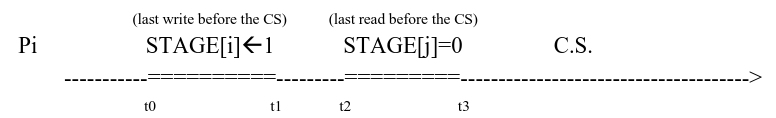
\includegraphics[width=0.8\linewidth]{images/aravinds-mutex-proof.png}
        %\captionof{figure}{MUTEX proof for Aravind’s algorithm.}
    \end{minipage}

Consider the timeline leading to $p_i$ entering the CS. At time $t_0$, $p_i$ writes 1 to \texttt{STAGE[i]}. At $t_1$, it performs its last read of \texttt{STAGE[j]} and finds it to be 0. If we assume $p_j$ also enters the CS, it must have also written \texttt{STAGE[j]}$\leftarrow$1 and read \texttt{STAGE[i]=0}. However, because $p_i$ has already written 1 to its stage register before reading $p_j$'s, and $p_j$ must do the same, their operations must overlap in a way that at least one process would see the other's \texttt{STAGE} as 1. This effectively blocks the concurrent entry. 
\end{demonstration}
\begin{corollary}
A useful corollary of this protocol is that the \texttt{DATE} registers are never written concurrently; because the updates occur within the unlock phase—which is protected by the mutual exclusion of the CS—only one process modifies these registers at any given time.
    \end{corollary}
\end{Thm}

\begin{Lemma}{Bounded DATE register into Aravind’s algorithm}{}
A reset of the \texttt{DATE} values occurs exactly every $n$ entries into the critical section.
\begin{demonstration}
This is because each entry into the CS increments the maximum date by one, and since the starting maximum is $n$ and the limit is $2n$, it takes $n$ steps to trigger the reset condition ($tmp\geq 2n$).
\end{demonstration}
\end{Lemma}

\begin{Lemma}{Bounded \texttt{DATE} register into Aravind’s algorithm}{}
During any single invocation of the lock routine by a process $p_i$, there can be at most one reset of the \texttt{DATE} registers.

This second lemma is vital for proving that the algorithm is starvation-free.

\begin{demonstration}
    If a reset occurs while $p_i$ is waiting, $p_i$ might see other processes leapfrog it. However, because a second reset cannot occur before $p_i$ enters, its progress is eventually guaranteed. In the worst-case scenario—where all $n$ processes invoke the lock simultaneously and $p_i$ has the highest index—all other $n-1$ processes might enter the CS before $p_i$, trigger a reset in their unlock phases, and potentially allow some processes to enter again before $p_i$ finally gains access.
\end{demonstration}
\end{Lemma}

\begin{Thm}{Bounded bypass proof for Aravind’s algorithm}{}
The algorithm satisfies the bounded bypass property with a bound of $2n-2$. This means a process can be bypassed by others at most $2n-2$ times before it is its turn to enter. 
\begin{demonstration}    
This bound is derived from the reset frequency: a process $p_n$ might have to wait for $n-1$ processes to finish their CS entries to trigger a reset, and potentially another $n-1$ entries after the reset before its own \texttt{DATE} becomes the "oldest" in the system.
\end{demonstration}
\end{Thm}

An improvement to Aravind's algorithm exists to tighten this bound to $n-1$. This revised version modifies the unlock phase. Instead of a simple increment and occasional global reset, the exiting process $p_i$ proactively decrements the \texttt{DATE} of any process $j$ that has a date greater than its own. It then sets its own \texttt{DATE} to $n$.


\begin{minipage}{\textwidth}
\begin{lstlisting}[mathescape]
unlock(i) :=
    $\forall$j$\neq$i if DATE[j] > DATE[i] then DATE[j] $\leftarrow$ DATE[j]-1
    DATE[i] $\leftarrow$ n
    STAGE[i] $\leftarrow$ 0
    FLAG[i] $\leftarrow$ down 
\end{lstlisting}
\captionof{lstlisting}{Improvement of Aravind’s algorithm.}
\end{minipage}\\

Because the lock protocol remains the same, this improved version still satisfies mutual exclusion. However, by constantly "shifting" the dates of waiting processes downward, it ensures a stricter FIFO-like (First-In-First-Out) order, reducing the maximum number of times a process can be bypassed.

\chapter{Concurrent Objects}
A \textit{concurrent object}\index{concurrent object} is defined as an entity that possesses a hidden internal implementation and a visible interface. This interface consists of a finite set of operations and a specification that describes its correct behaviors, typically in a sequential manner. When such an object is accessed by multiple processes simultaneously, it is termed a concurrent object.

\section{Semaphores}
The \textit{semaphore}\index{semaphore} is a fundamental shared synchronization object used to manage concurrency. It is essentially a shared counter, \texttt{S}, accessed through two atomic primitives: \texttt{up} and \texttt{down}. A semaphore is initialized to a non-negative value \texttt{s0} and must always remain greater than or equal to zero. The \texttt{up} operation atomically increases \texttt{S} by 1, while the \texttt{down} operation decreases it by 1, provided the value is not zero. If \texttt{S} is zero, the process invoking \texttt{down} is blocked and must wait until another process performs an \texttt{up}. This mechanism is primarily used to prevent busy waiting by suspending processes that cannot immediately proceed. The relationship between the operations and the counter is maintained by the invariant $S=s0+\#(S.up)-\#(S.down)$, where $\#$ denotes the number of completed operations.

In an ideal conceptual model, a semaphore consists of two underlying components: a counter that can become negative and a data structure, typically a FIFO queue, to store suspended processes. If the implementation counter is non-negative, it represents the actual value of the semaphore; if it is negative, its absolute value indicates the number of processes currently blocked in the queue. 

\begin{minipage}{\textwidth}
\begin{minipage}{0.45\textwidth}
\begin{lstlisting}[mathescape]
S.down() :=
    S.counter--
    if S.counter < 0 then
        enter into S.queue
        SUSPEND
    return
\end{lstlisting}
\end{minipage}
\hfill
\begin{minipage}{0.45\textwidth}
\begin{lstlisting}[mathescape]
S.up() :=
    S.counter++
    if S.counter $\leq$ 0 then
        activate a proc from S.queue
    return
\end{lstlisting}
\end{minipage}
\captionof{lstlisting}{Ideal semaphore implementation.}
\end{minipage}\\

A \textit{strong semaphore} utilizes a FIFO policy for unblocking, whereas a \textit{weak semaphore} one does not guarantee this order. A \textit{binary semaphore} is restricted to values of 0 or 1, meaning even the \texttt{up} operation can be blocking if the semaphore is already at 1.

The actual implementation of these primitives requires hardware support to ensure atomicity. This is achieved using a test\&set register—an atomic hardware instruction that sets a value while returning the old one—and by disabling interrupts to prevent the scheduler from preempting a process mid-operation. 

\begin{minipage}{\textwidth}
\begin{lstlisting}[mathescape]
Let t be a test&set register initialized at 0
\end{lstlisting}
\begin{minipage}{0.45\textwidth}
\begin{lstlisting}[mathescape]
S.down() :=
    Disable interrupts
    wait S.t.test&set() = 0
    S.counter--
    if S.counter < 0 then
        enter into S.queue
        S.t $\leftarrow$ 0
        Enable interrupts
        SUSPEND
    else S.t $\leftarrow$ 0
        Enable interrupts
    return
\end{lstlisting}
\end{minipage}
\hfill
\begin{minipage}{0.45\textwidth}
\begin{lstlisting}[mathescape]
S.up() :=
    Disable interrupts
    wait S.t.test&set() = 0
    S.count++
    if S.count $\leq$ 0 then
        activate a proc from S.queue
    S.t $\leftarrow$ 0
    Enable interrupts
    return
\end{lstlisting}
\end{minipage}
\captionof{lstlisting}{Actual semaphore implementation.}
\end{minipage}\\

In the implementation code, a process must first acquire a local lock (using test\&set) and disable interrupts before modifying the counter or the queue. Once the operation is complete, it resets the lock and re-enables interrupts. If a \texttt{down} operation results in a negative counter, the process is added to the queue and enters a \texttt{SUSPEND} state, relinquishing the processor until a corresponding \texttt{up} operation activates it.

\subsection{The Producer-Consumer Problem}
The \textit{Producer-Consumer problem}\index{producer-consumer} involves a shared FIFO buffer of size $k$. The internal representation of the buffer uses an array \texttt{BUF[0...k-1]} and two index variables, \texttt{IN} and \texttt{OUT}, which point to where items are inserted and removed circularly. In a single producer/consumer scenario, two semaphores are used: \texttt{FREE}, initialized at $k$, and \texttt{BUSY}, initialized at 0.

\begin{minipage}{\textwidth}
\begin{minipage}{0.45\textwidth}
\begin{lstlisting}[mathescape]
B.produce(v) :=
    FREE.down()
    BUF[IN] $\leftarrow$ v
    IN $\leftarrow$ (IN+1) mod k
    BUSY.up()
    return
\end{lstlisting}
\end{minipage}
\hfill
\begin{minipage}{0.45\textwidth}
\begin{lstlisting}[mathescape]
B.consume() :=
    BUSY.down()
    tmp $\leftarrow$ BUF[OUT]
    OUT $\leftarrow$ (OUT+1) mod k
    FREE.up()
return tmp
\end{lstlisting}
\end{minipage}
\captionof{lstlisting}{(Single) Producer/Consumer.}
\end{minipage}\\

The producer must perform a \texttt{FREE.down()} to ensure there is space before writing to \texttt{BUF[IN]} and incrementing \texttt{IN}. Conversely, the consumer performs a \texttt{BUSY.down()} to ensure there is data to read before accessing \texttt{BUF[OUT]} and incrementing \texttt{OUT}. This design ensures that the producer never overwrites unread data and the consumer never reads from an empty cell. However, reading or writing to the buffer can be computationally expensive, making mutual exclusion around the entire buffer a potential bottleneck.

When multiple producers or consumers are introduced, the variables \texttt{IN} and \texttt{OUT} must be protected from concurrent access to prevent two processes from using the same index. To allow for parallel access to different cells of the buffer, a more complex solution employs two arrays of atomic boolean registers, \texttt{BUSY} and \texttt{EMPTY}, to track the state of each individual cell. Two additional semaphores, \texttt{SP} and \texttt{SC} (both initialized to 1), are used to provide mutual exclusion specifically for the selection of the \texttt{IN} and \texttt{OUT} indices.

A "wrong" approach to this problem involves a producer taking an index \texttt{i = IN}, incrementing \texttt{IN} immediately, and then attempting to write.

\begin{minipage}{\textwidth}
\begin{minipage}{0.45\textwidth}
\begin{lstlisting}[mathescape]
B.produce(v) :=
    FREE.down()
    SP.down()
    i $\leftarrow$ IN
    IN $\leftarrow$ (i+1) mod k
    SP.up() 
    BUF[i] $\leftarrow$ v
    BUSY.up()
    return
\end{lstlisting}
\end{minipage}
\hfill
\begin{minipage}{0.45\textwidth}
\begin{lstlisting}[mathescape]
B.consume() :=
    BUSY.down()
    SC.down()
    o $\leftarrow$ OUT
    OUT $\leftarrow$ (o+1) mod k
    SC.up()
    tmp $\leftarrow$ BUF[o]
    FREE.up()
    return tmp
\end{lstlisting}
\end{minipage}
\captionof{lstlisting}{Wrong (Multiple) Producer/Consumer.}
\end{minipage}\\

If a very slow consumer is processing the first item while multiple quick producers fill the rest of the buffer, the indices can loop back around. Without proper cell-level checks (like the \texttt{while }$\neq$ \texttt{EMPTY[IN]} loop), a fast producer might attempt to overwrite a cell that the slow consumer is still reading, even if the general \texttt{FREE} semaphore allows the producer to proceed.

\begin{minipage}{\textwidth}
\begin{minipage}{0.45\textwidth}
\begin{lstlisting}[mathescape]
B.produce(v) :=
    FREE.down()
    SP.down()
    while $\lnot$EMPTY[IN] do
        IN $\leftarrow$ (IN+1) mod k
    i $\leftarrow$ IN
    EMPTY[i] $\leftarrow$ ff
    SP.up()
    BUF[i] $\leftarrow$ v
    FULL[i] $\leftarrow$ tt
    BUSY.up()
    return
\end{lstlisting}
\end{minipage}
\hfill
\begin{minipage}{0.45\textwidth}
\begin{lstlisting}[mathescape]
B.consume() :=
    BUSY.down()
    SC.down()
    while $\lnot$FULL[OUT] do
        OUT $\leftarrow$ (OUT+1) mod k
    o $\leftarrow$ OUT
    FULL[o] $\leftarrow$ ff
    SC.up()
    tmp $\leftarrow$ BUF[o]
    EMPTY[o] $\leftarrow$ tt
    FREE.up()
    return tmp
\end{lstlisting}
\end{minipage}
\captionof{lstlisting}{Correct (Multiple) Producer/Consumer.}
\end{minipage}\\

\subsection{The Readers/Writers Problem}
The \textit{Readers-Writers problem}\index{readers-writers} generalizes mutual exclusion by allowing multiple "readers" to access a resource (like a file) simultaneously, while "writers" require exclusive access. 

\begin{minipage}{\textwidth}
\begin{minipage}{0.45\textwidth}
\begin{lstlisting}[mathescape]
conc_read() :=
    begin_read()
    read()
    end_read()
\end{lstlisting}
\end{minipage}
\hfill
\begin{minipage}{0.45\textwidth}
\begin{lstlisting}[mathescape]
conc_write() :=
    begin_write()
    write()
    end_write()
\end{lstlisting}
\end{minipage}
\captionof{lstlisting}{Read/write operations on the file for the readers/writers problem.}
\end{minipage}\\

This leads to different priority schemes to manage access:
\begin{itemize}
    \item \textit{Weak Priority to Readers:} In this scheme, if a reader arrives while another reader is already active, it can enter even if a writer is waiting. A \texttt{GLOB\_MUTEX} semaphore manages access to the file, but only the first reader to arrive and the last reader to leave interact with it. A separate \texttt{R\_MUTEX} ensures that the reader count \texttt{R} is updated atomically.

\begin{minipage}{\textwidth}
\begin{lstlisting}[mathescape]
GLOB_MUTEX and R_MUTEX semaphores init. at 1
R a shared register init. at 0
\end{lstlisting}
\begin{minipage}{0.45\textwidth}
\begin{lstlisting}[mathescape]
begin_read() :=
    R_MUTEX.down()
    R++
    if R = 1 then GLOB_MUTEX.down()
    R_MUTEX.up()
    return
\end{lstlisting}
\end{minipage}
\hfill
\begin{minipage}{0.45\textwidth}
\begin{lstlisting}[mathescape]
end_read() :=
    R_MUTEX.down()
    R--
    if R = 0 then GLOB_MUTEX.up()
    R_MUTEX.up()
    return
\end{lstlisting}
\end{minipage}
\begin{minipage}{0.45\textwidth}
\begin{lstlisting}[mathescape]
begin_write() :=
    GLOB_MUTEX.down()
    return
\end{lstlisting}
\end{minipage}
\hfill
\begin{minipage}{0.45\textwidth}
\begin{lstlisting}[mathescape]
end_write() :=
    GLOB_MUTEX.up()
    return
\end{lstlisting}
\end{minipage}
\captionof{lstlisting}{Weak Priority to Readers.}
\end{minipage}\\
    
    \item \textit{Strong Priority to Readers:} This is a refinement where, upon a writer's termination, any waiting readers are prioritized over waiting writers. This is implemented by adding a \texttt{W\_MUTEX} that writers must acquire, effectively allowing readers to "queue up" and bypass writers more efficiently.

\begin{minipage}{\textwidth}
\begin{lstlisting}[mathescape]
GLOB_MUTEX, R_MUTEX and W_MUTEX semaphores init. at 1
R a shared register init. at 0
\end{lstlisting}
\begin{minipage}{0.45\textwidth}
\begin{lstlisting}[mathescape]
begin_read() :=
    R_MUTEX.down()
    R++
    if R = 1 then GLOB_MUTEX.down()
    R_MUTEX.up()
    return
\end{lstlisting}
\end{minipage}
\hfill
\begin{minipage}{0.45\textwidth}
\begin{lstlisting}[mathescape]
end_read() :=
    R_MUTEX.down()
    R--
    if R = 0 then GLOB_MUTEX.up()
    R_MUTEX.up()
    return
\end{lstlisting}
\end{minipage}
\begin{minipage}{0.45\textwidth}
\begin{lstlisting}[mathescape] 
begin_write() :=
    W_MUTEX.down()
    GLOB_MUTEX.down()
    return
\end{lstlisting}
\end{minipage}
\hfill
\begin{minipage}{0.45\textwidth}
\begin{lstlisting}[mathescape]
end_write() :=
    GLOB_MUTEX.up()
    W_MUTEX.up()
    return
\end{lstlisting}
\end{minipage}
\captionof{lstlisting}{Strong priority to Readers.}
\end{minipage}\\

    \item \textit{Weak Priority to Writers:} Here, the goal is to prevent writers from starving. If a writer is waiting, arriving readers are blocked. This is achieved using a \texttt{PRIO\_MUTEX}. When a writer wants to access the file, it increments a writer count \texttt{W}; the first writer to arrive grabs the \texttt{PRIO\_MUTEX}, which blocks any new readers from entering the system until all current writers have finished their work and the last writer releases the \texttt{PRIO\_MUTEX}.

\begin{minipage}{\textwidth}
\begin{lstlisting}[mathescape]
GLOB_MUTEX, PRIO_MUTEX, R_MUTEX and W_MUTEX semaphores init. at 1
R and W shared registers init. at 0
\end{lstlisting}
\begin{minipage}{0.45\textwidth}
\begin{lstlisting}[mathescape]
begin_read() :=
    PRIO_MUTEX.down()
    R_MUTEX.down()
    R++
    if R = 1 then GLOB_MUTEX.down()
    R_MUTEX.up()
    PRIO_MUTEX.up()
    return
\end{lstlisting}
\end{minipage}
\hfill
\begin{minipage}{0.45\textwidth}
\begin{lstlisting}[mathescape]
end_read() :=
    R_MUTEX.down()
    R--
    if R = 0 then GLOB_MUTEX.up()
    R_MUTEX.up()
    return
\end{lstlisting}
\end{minipage}
\begin{minipage}{0.45\textwidth}
\begin{lstlisting}[mathescape]
begin_write() :=
    W_MUTEX.down()
    W++
    if W = 1 then PRIO_MUTEX.down()
    W_MUTEX.up()
    GLOB_MUTEX.down()
    return
\end{lstlisting}
\end{minipage}
\hfill
\begin{minipage}{0.45\textwidth}
\begin{lstlisting}[mathescape]
end_write() :=
    GLOB_MUTEX.up()
    W_MUTEX.down()
    W--
    if W = 0 then PRIO_MUTEX.up()
    W_MUTEX.up()
    return
\end{lstlisting}
\end{minipage}
\captionof{lstlisting}{Weak priority to Writers.}
\end{minipage}\\

\end{itemize}

\section{Monitors}
In the evolution of concurrent programming, semaphores represented a foundational step, yet their low-level nature often makes them difficult to use correctly in complex systems. Monitors were introduced as a higher-level linguistic construct to provide a more structured approach to defining concurrent objects. A \textit{monitor}\index{monitor} is an abstract data type that guarantees mutual exclusion by design: at most one process can be active inside the monitor at any given time. This encapsulation simplifies the development of concurrent systems by moving the responsibility of mutual exclusion from the programmer to the programming language or runtime environment.

While mutual exclusion is handled automatically by the monitor, internal synchronization between processes—such as waiting for a specific condition to become true—is managed through condition variables. A \textit{condition} is an object that facilitates two primary operations: \texttt{wait} and \texttt{signal}. When a process invokes \texttt{C.wait()}, it suspends execution, joins the queue associated with condition \texttt{C}, and importantly, releases the mutual exclusion lock on the monitor so other processes can enter.

The \texttt{signal} operation behaves differently depending on the specific semantics of the monitor. If no processes are waiting on the condition, \texttt{signal} typically has no effect. However, if processes are suspended, the behavior branches into two main schools of thought. Under \textit{Hoare semantics}\index{Hoare semantics}, the signaling process immediately suspends itself and passes the monitor lock to the first process in the condition’s queue. This reactivated process has priority to re-enter or continue, and the signaling process only resumes once the monitor becomes free again. Conversely, \textit{Mesa semantics}\index{Mesa semantics} allow the signaling process to complete its current task or reach a suspension point before any signaled process is allowed to re-enter. In this model, the signal is more of a hint that the condition might be true, often requiring the signaled process to re-check the condition upon waking.

\subsection{Rendezvous through monitors}
A practical application of monitors is the implementation of a \textit{Rendezvous}\index{rendezvous} or \textit{Barrier}. This concurrent object is associated with $m$ control points, representing $m$ distinct processes. The goal is to ensure that no process can pass its control point until every other involved process has reached theirs.

\begin{minipage}{\textwidth}
\begin{lstlisting}[mathescape]
monitor RNDV :=
    cnt $\in$ {0,$\ldots$,m} init at 0
    
    condition B
    
    operation barrier() :=
        cnt++
        if cnt < m then B.wait()
                   else cnt $\leftarrow$ 0
        B.signal()
        return
\end{lstlisting}
\captionof{lstlisting}{Rendezvous through monitors.}
\end{minipage}\\

In a monitor-based implementation, a counter \texttt{cnt} tracks how many processes have arrived. Each process calls the \texttt{barrier()} operation. If the counter has not yet reached \texttt{m}, the process increments \texttt{cnt} and executes \texttt{B.wait()}, suspending itself. The last process to arrive (where \texttt{cnt} reaches \texttt{m}) does not wait; instead, it resets the counter to zero and calls \texttt{B.signal()} to wake the waiting processes. This pattern ensures that all processes are synchronized at a specific logical point before proceeding.

To understand the low-level mechanics of monitors, we can examine how they are implemented using semaphores. This requires managing several components: a \texttt{MUTEX} semaphore (initialized to 1) to ensure the monitor's primary mutual exclusion, and for each condition \texttt{C}, a semaphore \texttt{SEM}$_C$ (initialized to 0) along with a counter \texttt{$N_C$} to track suspended processes. To handle the priority requirements of Hoare semantics, an additional \texttt{PRIO} semaphore and an \texttt{$N_{PR}$} counter are used to manage processes that have performed a signal and are waiting to re-gain control of the monitor.

Every operation within the monitor is wrapped in a protocol. It begins with \texttt{MUTEX.down()}. Upon completion, the operation checks if any signaling processes are waiting (\texttt{$N_{PR}$ > 0}); if so, it releases one via \texttt{PRIO.up()}, otherwise, it releases the monitor via \texttt{MUTEX.up()}. 

\begin{minipage}{\textwidth}
\begin{lstlisting}[mathescape]
if N$_{PR}$ > 0 then PRIO.up() else MUTEX.up()
\end{lstlisting}
%\captionof{lstlisting}{Rendezvous through monitors.}
\end{minipage}\\

The \texttt{wait} and \texttt{signal} primitives are implemented as follows:
\begin{itemize}
    \item \texttt{C.wait()}: The process increments the count of waiting processes (\texttt{$N_C$}), releases the monitor (prioritizing signaling processes if they exist), and then blocks on \texttt{SEM}$_C$\texttt{.down()}. Once woken, it decrements \texttt{$N_C$}.

\begin{minipage}{\textwidth}
\begin{lstlisting}[mathescape]
C.wait() :=
    $N_C$++
    if $N_{PR}$ > 0 then PRIO.up() else MUTEX.up()
    SEM$_C$.down()
    $N_C$--
    return
\end{lstlisting}
%\captionof{lstlisting}{Rendezvous through monitors.}
\end{minipage}\\

    \item \texttt{C.signal()}: If there are processes waiting on the condition (\texttt{$N_C$ > 0}), the signaling process increments the priority count (\texttt{$N_{PR}$}), wakes a waiting process via \texttt{SEM}$_C$\texttt{.up()}, and then blocks itself on \texttt{PRIO.down()} to allow the signaled process to run. When it eventually resumes, it decrements \texttt{$N_{PR}$}.

\begin{minipage}{\textwidth}
\begin{lstlisting}[mathescape]
C.signal() :=
    if $N_C$ > 0 then $N_{PR}$++
                   SEM$_C$.up()
                   PRIO.down()
                   $N_{PR}$--
                   return
\end{lstlisting}
%\captionof{lstlisting}{Rendezvous through monitors.}
\end{minipage}\\
\end{itemize}

\subsection{Monitors for Readers/Writers}
The Readers/Writers problem can be elegantly solved using monitors by maintaining four state variables: Active Readers (\texttt{AR}), Waiting Readers (\texttt{WR}), Active Writers (\texttt{AW}), and Waiting Writers (\texttt{WW}).

\begin{minipage}{\textwidth}
\begin{lstlisting}[mathescape]
monitor RW_READERS :=
    AR, WR, AW, WW init at 0
    condition CR, CW
\end{lstlisting}
\begin{minipage}{0.45\textwidth}
\begin{lstlisting}[mathescape]
operation begin_read() :=
    WR++
    if AW$\neq$0 then CR.wait()
                 CR.signal()
    AR++
    WR--
\end{lstlisting}
\end{minipage}
\hfill
\begin{minipage}{0.45\textwidth}
\begin{lstlisting}[mathescape]
operation end_read() :=
    AR--
    if AR+WR=0 then CW.signal()
\end{lstlisting}
\end{minipage}
\begin{minipage}{0.45\textwidth}
\begin{lstlisting}[mathescape]
operation begin_write() :=
    if (AR+WR$\neq$0 OR AW$\neq$0) then
        CW.wait()
    AW++
\end{lstlisting}
\end{minipage}
\hfill
\begin{minipage}{0.45\textwidth}
\begin{lstlisting}[mathescape]
operation end_write() :=
    AW--
    if WR > 0 then
        CR.signal()
    else CW.signal()
\end{lstlisting}
\end{minipage}
\captionof{lstlisting}{Monitors Strong Priority to Readers.}
\end{minipage}\\

In the "Strong Priority to Readers" implementation, a reader can enter as long as no writer is currently active (\texttt{AW == 0}). If a writer is active, the reader increments \texttt{WR} and waits on \texttt{CR}. When a reader finishes (\texttt{end\_read}), if it is the last reader and no more readers are waiting, it signals a writer. This solution can lead to writer starvation, as a continuous stream of readers can keep the monitor in a state where \texttt{AW} remains zero while \texttt{AR} remains positive.

\begin{minipage}{\textwidth}
\begin{lstlisting}[mathescape]
monitor RW_WRITERS :=
    AR, WR, AW, WW init at 0
    condition CR, CW
\end{lstlisting}
\begin{minipage}{0.45\textwidth}
\begin{lstlisting}[mathescape]
operation begin_read() :=
    if WW+AW$\neq$0 then CR.wait()
                    CR.signal()
    AR++
\end{lstlisting}
\end{minipage}
\hfill
\begin{minipage}{0.45\textwidth}
\begin{lstlisting}[mathescape]
operation end_read() :=
    AR--
    if AR=0 then CW.signal()
\end{lstlisting}
\end{minipage}
\begin{minipage}{0.45\textwidth}
\begin{lstlisting}[mathescape]
operation begin_write() :=
    WW++
    if AR+AW$\neq$0 then CW.wait()
    AW++
    WW--
\end{lstlisting}
\end{minipage}
\hfill
\begin{minipage}{0.45\textwidth}
\begin{lstlisting}[mathescape]
operation end_write() :=
    AW--
    if WW > 0 then CW.signal()
              else CR.signal()
\end{lstlisting}
\end{minipage}
\captionof{lstlisting}{Monitors Strong Priority to Writers.}
\end{minipage}\\

Conversely, the "Strong Priority to Writers" version blocks new readers if there are any writers waiting (\texttt{WW + AW != 0}). In \texttt{begin\_write}, a writer increments \texttt{WW} and waits if any readers or writers are active. In \texttt{end\_write}, the finishing writer checks if there are other writers waiting and signals them first. Only if no writers remain does it signal the readers. This version risks starving the readers.

\begin{minipage}{\textwidth}
\begin{lstlisting}[mathescape]
monitor RW_FAIR :=
    AR, WR, AW, WW init at 0
condition CR, CW
\end{lstlisting}
\begin{minipage}{0.45\textwidth}
\begin{lstlisting}[mathescape]
operation begin_read() :=
    WR++
    if WW+AW$\neq$0 then CR.wait()
                    CR.signal()
    AR++
    WR--
\end{lstlisting}
\end{minipage}
\hfill
\begin{minipage}{0.45\textwidth}
\begin{lstlisting}[mathescape]
operation end_read() :=
    AR--
    if AR=0 then CW.signal()
\end{lstlisting}
\end{minipage}
\begin{minipage}{0.45\textwidth}
\begin{lstlisting}[mathescape]
begin_write() :=
    WW++
    if AR+AW$\neq$0 then CW.wait()
    AW++
    WW--
\end{lstlisting}
\end{minipage}
\hfill
\begin{minipage}{0.45\textwidth}
\begin{lstlisting}[mathescape]
operation end_write() :=
    AW--
    if WR > 0 then CR.signal()
              else CW.signal()
\end{lstlisting}
\end{minipage}
\captionof{lstlisting}{Monitors fair solution to Readers/Writers.}
\end{minipage}\\

A fair solution seeks to balance these interests. It dictates that during a read, new readers must wait if writers are already in the queue (\texttt{WW + AW != 0}). However, once a write operation finishes, it signals waiting readers to allow them to proceed. This prevents either group from monopolizing the resource indefinitely.


\subsection{The Dining Philosophers Problem}
The \textit{Dining Philosophers problem}\index{dining philosophers}, introduced by Dijkstra in 1965, illustrates the challenges of resource allocation and deadlock. $N$ philosophers sit at a circular table with $N$ chopsticks; each needs two chopsticks to eat.

\begin{figure}[ht]
    \centering
    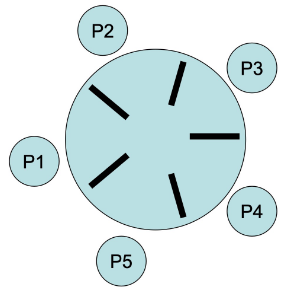
\includegraphics[width=0.4\linewidth]{images/dining-philosophers.png}
    \caption{Dining Philosophers}
    \label{fig:dining-philosophers}
\end{figure}

A naive semaphore solution, where each philosopher grabs the left chopstick and then the right, is susceptible to deadlock: if every philosopher picks up their left chopstick simultaneously, no one can pick up their right, and the system freezes. 

\begin{minipage}{\textwidth}
\begin{lstlisting}[mathescape]
semaphore chopstick[5] initialized to 1
\end{lstlisting}
\begin{lstlisting}[mathescape]
Philosopher(i) :=
    while(1) do
        chopstick[i].down()
        chopstick[(i+1)%N].down()
        // eat
        chopstick[(i+1)%N].up()
        chopstick[i].up()
\end{lstlisting}
\captionof{lstlisting}{Deadlock solution for Dining Philosophers Problem.}
\end{minipage}\\

Several strategies exist to break this symmetry and ensure a deadlock-free execution:
\begin{enumerate}
    \item \textit{Resource Hierarchy:} Assign a unique number to each fork. Philosophers must always attempt to pick up the lower-numbered fork first. This forces the last philosopher to pick up the forks in the opposite order of the others, breaking the circular wait.

\begin{minipage}{\textwidth}
\begin{lstlisting}[mathescape]
semaphore chopstick[5] initialized to 1
\end{lstlisting}
\begin{lstlisting}[mathescape]
Philosopher(i) :=
    Repeat
    think;
    if (i < N-1) then
        fork[i].down();
        fork[i+1].down();
    else
        fork[0].down();
        fork[N-1].down();
    eat;
    fork[(i+1)%N].up();
    fork[i].up();
\end{lstlisting}
\captionof{lstlisting}{Resource Hierarchy solution for Dining Philosophers Problem.}
\end{minipage}\\

    \item \textit{Parity-Based Selection:} Odd-numbered philosophers pick up the left fork then the right, while even-numbered philosophers pick up the right then the left. This prevents the circular dependency required for deadlock.

\begin{minipage}{\textwidth}
\begin{lstlisting}[mathescape]
semaphore chopstick[5] initialized to 1
\end{lstlisting}
\begin{lstlisting}[mathescape]
Philosopher(i) :=
    Repeat
        think;
        if (i % 2 == 0) then
            fork[i].down();
            fork[(i+1)%N].down();
        else
            fork[(i+1)%N].down();
            fork[i].down();
        eat;
        fork[(i+1)%N].up();
        fork[i].up();
\end{lstlisting}
\captionof{lstlisting}{Parity-Based Selection solution for Dining Philosophers Problem.}
\end{minipage}\\

    \item \textit{Admission Control:} Use a "table" semaphore initialized to $N-1$. By allowing only four philosophers at a table of five, at least one philosopher is guaranteed to have access to two chopsticks.

\begin{minipage}{\textwidth}
\begin{lstlisting}[mathescape]
semaphores fork[N] all initialized at 1
semaphore table initialized at N-1
\end{lstlisting}
\begin{lstlisting}[mathescape]
Philosopher(i) :=
    Repeat
        think;
        table.down();
        fork[i].down();
        fork[(i+1)%N].down();
        eat;
        fork[(i+1)%N].up();
        fork[i].up();
        table.up() 
\end{lstlisting}
\captionof{lstlisting}{Admission Control solution for Dining Philosophers Problem.}
\end{minipage}\\

    \item \textit{Monitor-Based State Testing:} This solution uses a monitor to track the state of each philosopher (thinking, hungry, or eating). A philosopher only moves to the eating state if both neighbors are not currently eating. This is managed via a \texttt{test(i)} function. If a philosopher cannot eat, they wait on a condition variable \texttt{self[i]}. When a neighbor finishes eating and calls \texttt{Putdown}, they execute test on their neighbors, signaling any who are hungry and now able to eat. This approach ensures that the "hungry" state is correctly transitioned only when the necessary resources are actually available.
    
\begin{minipage}{\textwidth}
\begin{lstlisting}[mathescape]
monitor DP
    status state[N] all initialized at thinking;
    condition self[N];

    Pickup(i) :=
        state[i] = hungry;
        test(i);
        if (state[i] != eating) then self[i].wait;
    
    Putdown(i) :=
        state[i] = thinking;
        test((i+1)%N);
        test((i-1)%N);
    
    test(i) :=
        if (state[(i+1)%N] != eating && state[(i-1)%N] != eating
            && state[i] == hungry)
        then state[i] = eating;
             self[i].signal();
\end{lstlisting}
\captionof{lstlisting}{Monitor-Based State Testing solution for Dining Philosophers Problem.}
\end{minipage}\\
    
\end{enumerate}

\chapter{Software Transactional Memory}
\textit{Software Transactional Memory (STM)}\index{software transactional memory (STM)} is a high-level synchronization mechanism designed to simplify concurrent programming. By providing an abstraction similar to database transactions, STM allows developers to define blocks of code that must execute atomically without having to manually manage low-level synchronization primitives like locks.

An STM system groups together parts of the application code that must appear atomic to an external observer. Unlike traditional monitors, where atomicity is tied to the definition of an object, STM allows atomicity to be application-dependent. Furthermore, unlike database transactions which are often limited to SQL-like queries, STM transactions can consist of any arbitrary code accessing shared atomic objects.

A \textit{transaction}\index{transaction} is defined as an atomic unit of computation that accesses "$t$-objects" (atomic objects used within transactions). It is assumed that any transaction will successfully terminate if executed in isolation. A \textit{program} in this context consists of multiple sequential processes that alternate between transactional and non-transactional code. The role of the \textit{STM system} is to act as an online algorithm ensuring that all transactional code executes with the appearance of atomicity.

To maintain efficiency, STM systems typically employ \textit{optimistic execution}, where multiple transactions run simultaneously. If two transactions conflict (e.g., both access the same object and at least one modifies it), the system must ensure they can still be totally ordered. If a correct ordering is impossible, a transaction is aborted and may be re-executed or the parent process notified. This introduces the possibility of unbounded delays, which is the "price" of synchronization.

Conceptually, a transaction involves three distinct phases:
\begin{enumerate}
    \item \textit{Read Phase:} Reading values from atomic registers.
    \item \textit{Local Computation:} Processing data within a local workspace.
    \item \textit{Write Phase:} Updating shared memory with new values.
\end{enumerate}
    
Maintaining the consistency of shared memory is critical; if any inconsistency is detected during execution, the transaction must abort. Most implementations use a local working space to isolate changes until they are ready to be committed. When a shared register is first read, its value is copied locally. Subsequent reads use this local copy. Writes only modify the local copy and are only pushed to shared memory at the end of the transaction if the commit is successful.

The standard STM interface provides four operations:
\begin{itemize}
    \item \texttt{begin}$_T$\texttt{()}: Initializes local control variables and timestamps.
    \item \texttt{X.read}$_T$\texttt{()}: Reads the implementation register \texttt{XX}. If it is the first read, it copies the value to the local workspace.
    \item \texttt{X.write}$_T$\texttt{(v)}: Updates the local copy of the register with value \texttt{v}.
    \item \texttt{try\_to\_commit}$_T$\texttt{()}: Validates the transaction's read set and determines if it can safely commit its changes to shared memory.
\end{itemize}

\section{Opacity}
A common approach to STM consistency is \textit{opacity}\index{opacity}, which requires that all committed transactions, as well as the read prefixes of all aborted transactions, appear to execute in a sequential order that respects their real-time occurrence. This prevents transactions from ever reading from an inconsistent global state.

\textit{Transactional Locking 2 (TL2)}\index{transactional locking 2 (TL2)} is a logical clock-based STM system that ensures opacity. It utilizes a global atomic \texttt{CLOCK} register. Every application register \texttt{X} is represented by an implementation pair \texttt{XX} containing the value (\texttt{XX.val}) and the date of its last update (\texttt{XX.date}).

In TL2, each transaction $T$ maintains:
\begin{itemize}
    \item \texttt{lc(XX)}: Local copies of implementation registers.
    \item \texttt{read\_set(T)} and \texttt{write\_set(T)}: Sets tracking accessed registers.
    \item \texttt{birthdate(T)}: The value of \texttt{CLOCK} at the start of the transaction.
\end{itemize}
    
Consistency is maintained by ensuring that for any read, the register's version date is less than the transaction's birthdate (\texttt{XX.date < birthdate(T)}). During \texttt{try\_to\_commit}$_T$\texttt{()}, the system locks all registers in the read and write sets, re-validates their dates against the birthdate, and—if valid—increments the global clock to provide a new timestamp for the written values. To prevent deadlocks during the locking phase, registers are always locked according to a predefined total order.

\begin{minipage}{\textwidth}
\begin{minipage}{0.45\textwidth}
\begin{lstlisting}[mathescape]
begin$_T$() :=
    read_set(T), write_set(T) $\leftarrow$ $\emptyset$
    birthdate(T) $\leftarrow$ CLOCK+1
\end{lstlisting}
\end{minipage}
\hfill
\begin{minipage}{0.45\textwidth}
\begin{lstlisting}[mathescape]
X.write$_T$(v) :=
    if lc(XX)=$\perp$ then lc(XX) $\leftarrow$ newloc
    lc(XX).val $\leftarrow$ v
    write_set(T) $\leftarrow$ write_set(T) $\cup$ {X}
\end{lstlisting}
\end{minipage}
\begin{minipage}{0.45\textwidth}
\begin{lstlisting}[mathescape]
X.read$_T$() :=
    if lc(XX)$\neq\perp$ then return lc(XX).val
    lc(XX) $\leftarrow$ XX
    if lc(XX).date $\geq$ birthdate(T) then ABORT
    read_set(T) $\leftarrow$ read_set(T) $\cup$ {X}
    return lc(XX).val
\end{lstlisting}
\end{minipage}
\hfill
\begin{minipage}{0.45\textwidth}
\begin{lstlisting}[mathescape]
try_to_commit$_T$() :=
    lock all read_set(T) $\cup$ write_set(T)
    $\forall$ X $\in$ read_set(T)
        if XX.date $\geq$ birthdate(T)
        then release all locks
            ABORT
    tmp $\leftarrow$ CLOCK.fetch&add(1)+1
    $\forall$ X $\in$ write_set(T)
        XX $\leftarrow$ $\langle$lc(XX).val, tmp$\rangle$
    release all locks
    COMMIT
\end{lstlisting}
\end{minipage}
\captionof{lstlisting}{A Logical Clock based STM system.}
\end{minipage}\\

\section{Virtual World Consistency}
Opacity is a strong condition that can be restrictive. \textit{Virtual World Consistency (VWC)}\index{virtual world consistency (VWC)} is a more liberal property. While it still requires committed transactions to be linearizable, it only requires aborted transactions to be consistent with their own causal past (their "virtual world") rather than a single global history. The causal past of a transaction \texttt{T} includes any committed transaction \texttt{T'} that \texttt{T} has read from, along with all transactions that preceded \texttt{T'}.

\begin{figure}[ht]
    \centering
    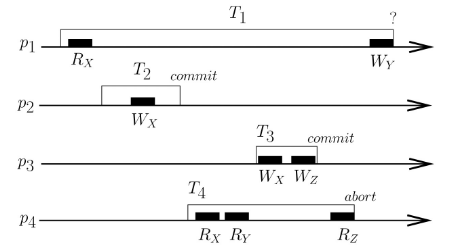
\includegraphics[width=0.5\linewidth]{images/virtual-world-consintency.png}
    \caption{Virtual World Consistency example.}
    \label{fig:virtual-world-consintency}
\end{figure}

Consider an example with four transactions: $T_1$, $T_2$, $T_3$, and $T_4$ (Figure \ref{fig:virtual-world-consintency}). In an execution where $T_1$ and $T_2$ are sequential and $T_3$ is concurrent, opacity might force $T_1$ to abort if $T_4$ (an aborted transaction) reads an inconsistent value between $T_2$ and $T_3$. However, under VWC, $T_1$ can commit because $T_4$ only needs to be consistent relative to its specific causal dependencies (e.g., $T_2<r_pref(T_4)$), even if it cannot be globally ordered with $T_3$.


To implement VWC efficiently and avoid the bottleneck of a single global logical clock, a \textit{vector clock-based STM}\index{vector clock-based STM} can be used. In this system, each of the $m$ registers stores a vector clock \texttt{XX.depend[1...m]}. \texttt{XX.depend[X]} represents the sequence number of the current value of \texttt{X}, while \texttt{XX.depend[Y]} tracks the sequence number of register \texttt{Y} upon which the current value of \texttt{X} depends.

Processes maintain their own local vector clocks (\texttt{p\_depend}), which are used to initialize a transaction's local dependency vector (\texttt{t\_depend}$_T$).

\begin{minipage}{\textwidth}
\begin{minipage}{0.45\textwidth}
\begin{lstlisting}[mathescape]
begin$_T$(i) :=
    read_set(T), write_set(T) $\leftarrow$ $\emptyset$
    t_depend$_T$ $\leftarrow$ p_depend$_i$

X.read$_T$(i) :=
    if lc(XX)=$\perp$ then
        lc(XX) $\leftarrow$ newloc
        lc(XX) $\leftarrow$ XX
        read_set(T) $\leftarrow$ read_set(T) $\cup$ {X}
        t_depend$_T$[X] $\leftarrow$ lc(XX).depend[X]
        if $\exists$ Y $\in$ read_set(T) s.t.
            t_depend$_T$[Y] < lc(XX).depend[Y]
        then ABORT
        $\forall$ Y $\notin$ read_set(T) do
            t_depend$_T$[Y] $\leftarrow$ max{t_depend$_T$[Y],
                               lc(XX).depend[Y]}
    return lc(XX).val
\end{lstlisting}
\end{minipage}
\hfill
\begin{minipage}{0.45\textwidth}
\begin{lstlisting}[mathescape]
X.write$_T$(i,v) :=
    if lc(XX)=$\perp$ then lc(XX) $\leftarrow$ newloc
    lc(XX).val $\leftarrow$ v
    write_set(T) $\leftarrow$ write_set(T) $\cup$ {X}

try_to_commit$_T$(i) :=
    lock all read_set(T) $\cup$ write_set(T)
    if $\exists$ Y $\in$ read_set(T) s.t.
        t_depend$_T$[Y] < YY.depend[Y]
    then release all locks
        ABORT
    $\forall$ X $\in$ write_set(T) do
        t_depend$_T$[X] $\leftarrow$ XX.depend[X]+1
    $\forall$ X $\in$ write_set(T) do
        XX $\leftarrow$ $\langle$lc(XX).val, t_depend$_T$$\rangle$
    release all locks
    p_depend$_i$ $\leftarrow$ t_depend$_T$
    COMMIT 
\end{lstlisting}
\end{minipage}
\captionof{lstlisting}{A Vector clock based STM system.}
\end{minipage}\\

The consistency check during \texttt{X.read}$_T$\texttt{()} ensures that the value of \texttt{X} does not depend on a version of any register \texttt{Y} that is "newer" than what the transaction has already seen (\texttt{t\_depend}$_T$\texttt{[Y] < lc(XX).depend[Y]}). If this check passes, \texttt{t\_depend}$_T$ is updated to include the new dependencies from the register just read. This approach allows for higher concurrency by localizing consistency checks to relevant dependencies rather than a global timeline.

\chapter{Atomicity}
This chapter explores the formal foundations of \textit{atomicity}\index{atomiticy}, a fundamental consistency condition in concurrent systems. As introduced in earlier contexts, atomicity allows us to judge the correctness of a concurrent implementation by relating it to a sequential execution. This formal perspective, often referred to as linearizability when applied to any concurrent object, provides a framework for reasoning about processes that access shared resources.

We consider a system composed of a set of $n$ sequential processes, $p_1,\ldots p_n$, which access $m$ concurrent objects, $X_1,\dots,X_m$. Processes interact with these objects by invoking operations of the form $X_i$\texttt{.op(args)(ret)}. To model the duration and concurrency of these operations, each invocation by a process $p_j$ is represented by two distinct events:
\begin{itemize}
    \item An invocation event: \texttt{inv[}$X_i$\texttt{.op(args) by }$p_j$\texttt{]}
    \item A response event: \texttt{res[}$X_i$\texttt{.op(ret) to }$p_j$\texttt{]}
\end{itemize}

A \textit{history}\index{history} (or \textit{trace}), denoted as $\widehat{H}=(H,<_H)$, consists of a set of these events $H$ and a total order $<_H$ defined over them. This order must satisfy the basic requirement that every response event follows its corresponding invocation event. The semantics of the system or its individual objects are defined as the set of all possible valid traces they can produce.

Histories can be classified based on their structure:
\begin{itemize}
    \item \textit{Sequential History:} A history where events appear in strictly alternating pairs: $inv,res,inv,res,\ldots$ In such a history, every response is the immediate successor of its corresponding invocation. Because of this structure, a sequential history can be simplified and represented merely as a sequence of operations.
    \item \textit{Complete vs. Partial:} A history is complete if every invocation event is eventually matched by a corresponding response event. If some invocations remain "hanging" without a return, the history is considered partial.
\end{itemize}

\section{Linearizability}
\textit{Linearizability}\index{linearizability} is the gold standard for correctness in concurrent object design. A complete history $\widehat{H}$ is defined as linearizable if there exists a equivalent sequential history $\widehat{S}$ that satisfies three specific conditions:
\begin{enumerate}
    \item \textit{Object Semantics:}\index{object semantics} For every object $X$, the restriction of $\widehat{S}$ to $X$ (denoted $\widehat{S}|_X$) must belong to the sequential specification (semantics) of that object.
    \begin{equation*}
        \forall X \widehat{S}|_X\in semantics(X)
    \end{equation*}
    \item \textit{Process Consistency:}\index{process consistency} For every process $p$, the order of operations in $\widehat{H}$ as seen by $p$ must be identical to the order in $\widehat{S}$ (i.e., $\widehat{H}|p=\widehat{S}|p$).
    \begin{equation*}
        \forall p \widehat{H}|_p = \widehat{S}|_p
    \end{equation*}
    \item \textit{Real-Time Order Preservance:}\index{real-time order preservance} If an operation $op$ completes in $\widehat{H}$ before another operation $op'$ begins (meaning $res[op]<_H inv[op']$), then $op$ must also precede $op'$ in the sequential history $\widehat{S}$ ($res[op]<_S inv[op']$).
    \begin{equation*}
        \textit{if }res[op] <_H inv[op'],\textit{ then }res[op] <_S inv[op']
    \end{equation*}
\end{enumerate}

To formalize the third condition, we define a binary relation $\longrightarrow_H$ such that $(op,op')\in\longrightarrow_H$ (written $op\longrightarrow_H op'$) if and only if $res[op]<_H inv[op']$. Linearizability essentially requires that the sequential order $\longrightarrow_S$ is a superset of the real-time precedence order $\longrightarrow_H$ ($\longrightarrow_H \subseteq \longrightarrow_S$).

\begin{Example}{A Linearizable Queue}{}
    Consider a queue $Q$ accessed by two processes. Process $p_1$ enqueues $a$ and $b$ (\texttt{Q.enq(a)} and \texttt{Q.enq(b)}), while process $p_2$ enqueues $c$ and performs a dequeue (\texttt{Q.deq->a}).

    \begin{minipage}{\textwidth}
        \centering
        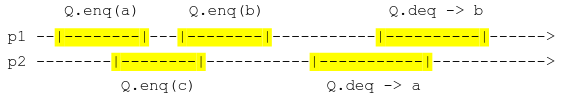
\includegraphics[width=0.8\linewidth]{images/linearizable-queue-example.png}
        \captionof{figure}{Linearizable Queue Timeline.}
    \end{minipage}

    The physical timeline might show these operations overlapping. For instance, $p_2$'s \texttt{enq(c)} might start after $p_1$'s \texttt{enq(a)} has started but before it finishes. If $p_2$ eventually dequeues $a$, we must find a sequential order that makes sense. One such linearization is:
    \begin{equation*}
        [Q.enq(a)]\rightarrow[Q.enq(b)]\rightarrow[Q.enq(c)]\rightarrow[Q.deq\rightarrow a]\rightarrow[Q.deq\rightarrow b].        
    \end{equation*}
This sequence satisfies the FIFO (First-In-First-Out) semantics of a queue and respects the order in which individual processes issued their commands.

However, certain histories are not linearizable. If $p_2$ dequeues $a$ in a context where \texttt{enq(a)} clearly happened after another completed operation that remains in the queue, or if the real-time order is violated (e.g., $p_2$ dequeues a but \texttt{enq(a)} starts only after $p_2$'s dequeue has already finished), the history cannot be linearized.

    \begin{minipage}{\textwidth}
        \centering
        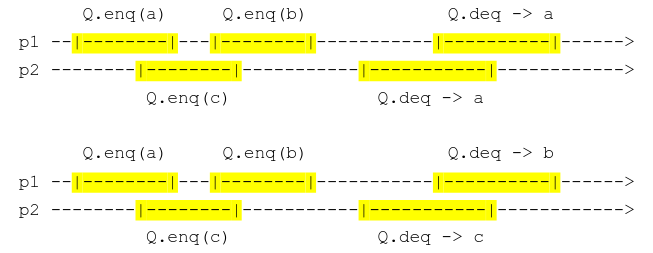
\includegraphics[width=0.7\linewidth]{images/non-linearizable.png}
        \captionof{figure}{Non-Linearizable Queue Timeline.}
    \end{minipage}
\end{Example}

\subsection{Compositionality of Linearizability}
\begin{Thm}{Compositionality}{}
    One of the most powerful properties of linearizability is \textit{compositionality}\index{compositionality} (also known as the \textit{locality property} in the literature). This property states that a history $\widehat{H}$ is linearizable if and only if its restriction to every individual object $X$ ($\widehat{H}|_X$) is linearizable. 

    This allows system designers to verify the correctness of each object in isolation, guaranteed that their combination will also be correct.

    \begin{demonstration}
    To prove this, we assume that for every object $X$, there is a linearization $\widehat{S}_X$. This $\widehat{S}_X$ defines a total order on operations for that specific object, which we call $\longrightarrow_X$. We then define a global relation $\longrightarrow$ as the union of the real-time order $\longrightarrow_H$ and all individual object orders $\longrightarrow_X$:
    \begin{equation*}
        \longrightarrow =\longrightarrow_H \cup \bigcup_X \longrightarrow_X
    \end{equation*}

    The core of the proof lies in showing that this relation $\longrightarrow$ is acyclic:
    \begin{enumerate}
        \item \textit{No self-loops:} An operation cannot precede itself ($res(op)<inv(op)$ is impossible).
        \item \textit{No 2-cycles:} If $op\longrightarrow op'\longrightarrow op$, it cannot be that both edges are from the same $\longrightarrow_X$ or $\longrightarrow_H$ (as those are acyclic). It also cannot be across different objects $X$ and $Y$. The only possibility is $op\longrightarrow_X op'\longrightarrow_H op$. But if $op'\longrightarrow_H op$, then $res(op')<_H inv(op)$. In a linearization of $X$, this would force $op'\longrightarrow_X op$, creating a cycle in the sequential order of $X$, which is a contradiction.
        \item \textit{No larger cycles:} By induction and the properties of the shortest cycle, we can show that any cycle would eventually force a contradiction of the real-time order $\longrightarrow_H$ or the individual object semantics.
    \end{enumerate}

    Since $\longrightarrow$ is a Directed Acyclic Graph (DAG), it admits a topological order ($\longrightarrow '$). We can then construct our global sequential history $\widehat{S}$ by arranging operations according to this topological order. This constructed history $\widehat{S}$ will naturally satisfy object semantics (matching $\widehat{S}_X$), process consistency (matching $p$'s sequential nature), and real-time order (since $\longrightarrow_H \subseteq \longrightarrow \subseteq \longrightarrow '$).
\end{demonstration}
\end{Thm}

\begin{Example}{Composition of a Queue and a Stack}{}
    Consider processes $p_1$, $p_2$, $p_3$ accessing a Queue $Q$ and a Stack $S$.
    \begin{itemize}
        \item $p_1$ interacts with $Q$ and $S$.
        \item $p_2$ interacts with $Q$.
        \item $p_3$ interacts with $S$.
    \end{itemize}

    \begin{minipage}{\textwidth}
        \centering
        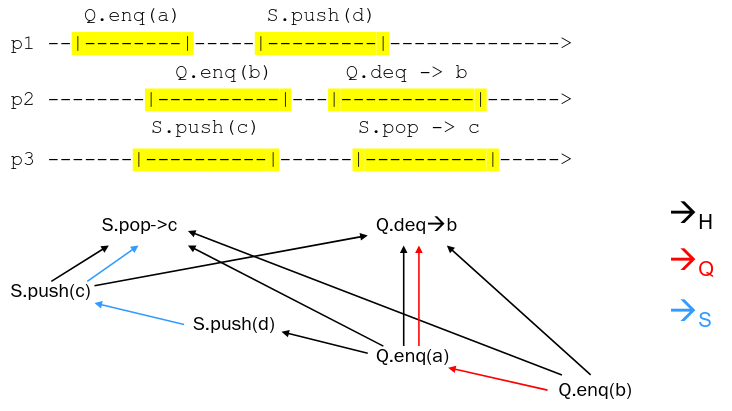
\includegraphics[width=0.7\linewidth]{images/compositionality-example.png}
        \captionof{figure}{Compositionality Timeline and DAG.}
    \end{minipage}
    
    By verifying that the operations on $Q$ are linearizable and the operations on $S$ are linearizable independently, compositionality ensures the entire interleaved execution is linearizable. We can find a total order (e.g., \texttt{Q.enq(b),Q.enq(a),S.push(d),S.push(c),...}) that respects the internal logic of both the stack and the queue while maintaining the real-time precedence of the original execution.
\end{Example}

\section{Alternatives to Atomicity}
While linearizability is robust, other consistency models exist, often relaxing the strict real-time requirement to allow for more performance or different system behaviors.

\subsection{Sequential Consistency}
\textit{Sequential consistency}\index{sequential consistency} is a more "generous" or "lazy" version of linearizability. It relaxes the third condition: instead of respecting the global real-time order $\longrightarrow_H$, it only respects the process order $\longrightarrow_{proc}$.

\begin{Definition}{Complete sequential history}{}
    A complete history $\widehat{H}$ is \textit{sequentially consistent} if there exists a sequential history $\widehat{S}$ such that object semantics and process orders are preserved, but only $op\longrightarrow_{proc} op' \implies op\longrightarrow_S op'$.

    \begin{enumerate}
        \item $\forall X \widehat{S}|_X \in semantics(X)$
        \item $\forall p \widehat{H}|_p = \widehat{S}_p$
        \item $\longrightarrow_{proc} \subseteq \longrightarrow_S$
    \end{enumerate}
\end{Definition}

\begin{Example}{Sequential non-linearizable history}{}
    An example of a history that is sequentially consistent but not linearizable is a queue where $p_1$ enqueues $a$ and $p_2$ subsequently enqueues $b$ and then dequeues $b$. 

    \begin{equation*}
        [Q.enq(a)()\textit{ by }p_1][Q.enq(b)()\textit{ by }p_2][Q.deq()(b)\textit{ to }p_2]
    \end{equation*}
    
    In real-time, $a$ was in the queue first. Linearizability would require $a$ to be dequeued first. Sequential consistency, however, allows us to "reorder" the enqueues in our minds so that $b$ was enqueued before $a$, thus satisfying the queue semantics.
\end{Example}

Sequential consistency is not compositional. Two histories can be individually sequentially consistent, but their composition may not be. 

\begin{Example}{Non-compositional sequential consistency}{}
\begin{align*}
    &p_1: Q.enq(a); Q’.enq(b’); Q’.deq()\rightarrow b’\\
    &p_2: Q’.enq(a’); Q.enq(b); Q.deq()\rightarrow b
\end{align*}

If two processes $p_1$ and $p_2$ interact with two different queues $Q$ and $Q'$ in a cross-dependency (e.g., $p_1$ enqueues to $Q$ then $Q'$, $p_2$ enqueues to $Q'$ then $Q$), the local sequential orderings required to satisfy each queue might contradict each other when combined into a single global order.    
\end{Example}

\subsection{Serializability}
Commonly used in database systems, \textit{serializability}\index{serializability} shifts the focus from processes to transactions.

Operations are grouped into transactions, which end with either a \texttt{commit(t)} or \texttt{abort(t)} event.

\begin{Definition}{Serializability}{}
    A history is \textit{serializable} if there is a sequential history $\widehat{S}$ (consisting of only committed transactions) that preserves object semantics and the transaction order $\longrightarrow_{trans}$ (where one transaction finishes before another begins).

    \begin{enumerate}
        \item $\forall X \widehat{S}|_X \in semantics(X)$
        \item $S=\{e\in H: e\in t\in committedTrans(\widehat{H})\}$
        \item $\longrightarrow_{trans} \subseteq \longrightarrow_S$
    \end{enumerate}
\end{Definition}

Like sequential consistency, serializability is more flexible than linearizability because it focuses on the logical order of transactions rather than the wall-clock time of every individual event. However, it shares the same critical flaw: it is not compositional. Combining two serializable database systems does not automatically result in a serializable global system without additional coordination.


\chapter{MUTEX-free Concurrency}
Traditional concurrent systems rely heavily on critical sections and locks to ensure safety. However, this approach introduces several systemic risks. If locks are implemented with improper granularity, they can lead to performance bottlenecks by unnecessarily reducing concurrency. More critically, the delay or failure of a single process—such as a process crashing while holding a lock—can stall the entire system indefinitely.

\textit{Mutex-freedom}\index{mutex-freedom} addresses these issues by ensuring that the only atomic operations used are those provided directly by the hardware (such as atomic Read/Write registers, Compare-and-Swap, or Fetch-and-Add). Because these systems do not use traditional critical sections, we require a new set of liveness properties to define progress. These properties are particularly robust in the face of process crashes (fail-stop failures), as asynchrony makes it impossible for the system to distinguish between a crashed process and one that is simply delayed.

The four primary progress conditions are:
\begin{enumerate}
    \item \textit{Obstruction-freedom:}\index{obstruction-freedom} This is the weakest condition. It guarantees that an operation will terminate if it eventually executes in isolation (i.e., without contention from other processes for a sufficient period).
    \item \textit{Non-blocking (Lock-free):}\index{non-blocking (lock-free)} This ensures that at least one of the active operations on an object will eventually terminate. While individual processes might still face starvation, the system as a whole always makes progress. This is analogous to deadlock-freedom in lock-based systems.
    \item \textit{Wait-freedom:}\index{wait-freedom} This is the strongest condition, ensuring that every operation invoked by a process will eventually terminate, regardless of the speed or interference of other processes. This is the mutex-free equivalent of starvation-freedom.
    \item \textit{Bounded Wait-freedom:}\index{bounded wait-freedom} This is a stronger version of wait-freedom where there is a known upper bound on the number of steps a process must take before finishing. This mirrors the concept of bounded bypass.
\end{enumerate}

\section{Wait-free Splitter}
A \textit{splitter}\index{splitter} is a fundamental building block in distributed computing used to "partition" processes. It provides a single operation, \texttt{dir(i)}, which returns one of three values: $L$ (Left), $R$ (Right), or $S$ (Stop).

For a splitter to be valid, it must satisfy three properties:
\begin{itemize}
    \item \textit{Validity:} It must return $L$, $R$, or $S$.
    \item \textit{Concurrency:} If $n$ processes invoke the splitter, at most $n-1$ can go \texttt{Left}, at most $n-1$ can go \texttt{Right}, and at most one process can obtain the \texttt{Stop} value.
    \item \textit{Wait-freedom:} Every invocation must terminate.
\end{itemize}

In a "solo" execution where only one process enters the splitter, that process is guaranteed to receive the $S$ value. This makes the splitter highly effective for resource allocation or leadership election in a distributed environment.

The implementation uses two atomic registers: \texttt{DOOR} (a boolean initialized to 1) and \texttt{LAST} (initialized to a default process index).

\begin{minipage}{\textwidth}
\begin{lstlisting}[mathescape]
DOOR: MRMW boolean atomic register initialized at 1
LAST: MRMW atomic register initialized at whatever process index
\end{lstlisting}
\begin{lstlisting}[mathescape]
dir(i) :=
    LAST $\leftarrow$ i
    if DOOR = 0 then return R
                else DOOR $\leftarrow$ 0
                    if LAST = i then return S
                                else return L
\end{lstlisting}
\captionof{lstlisting}{Wait-free Splitter.}
\end{minipage}\\

The logic follows a specific sequence: a process first announces its arrival by writing its \texttt{ID} to \texttt{LAST}. It then checks the \texttt{DOOR}. If the door is already closed (\texttt{DOOR = 0}), it immediately exits to the Right (\texttt{R}). If the door is open, the process closes it and then checks if it is still the "last" process to have written to \texttt{LAST}. If its \texttt{ID} remains in \texttt{LAST}, it stops (\texttt{S}); otherwise, it concludes that another process has overtaken it and moves to the Left (\texttt{L}).

\begin{Thm}{Soundness proof for wait-free Splitter}{}
    The termination and validity of the splitter are straightforward due to the lack of loops. 
    \begin{demonstration}
    The concurrency property is proved through three observations:
    \begin{itemize}
        \item Not everyone can go Right: To receive \texttt{R}, a process must find the \texttt{DOOR} at 0. The first process to find the door at 1 will close it and cannot receive \texttt{R}.
        \item Not everyone can go Left: Consider the last process $p_i$ to write to the \texttt{LAST} register. If $p_i$ finds the door closed, it goes \texttt{R}. If it finds the door open, it will inevitably find \texttt{LAST = i} (since no one writes after it) and will receive \texttt{S}.
        \item At most one process stops: Suppose $p_i$ is the first process to receive \texttt{S}. This means $p_i$ found \texttt{LAST = i} during its second check. Any process $p_j$ that wrote to \texttt{LAST} before $p_i$ will find \texttt{LAST} has changed (to i or a later value) and will go \texttt{L}. Any process $p_j$ that tries to write to \texttt{LAST} after $p_i$ has already closed the door will find \texttt{DOOR = 0} and go \texttt{R}.
    \end{itemize}
    \end{demonstration}
\end{Thm}

\section{Obstruction-free Timestamp Generator}
A \textit{timestamp generator}\index{timestamp generator} provides a \texttt{get\_ts} operation that must ensure:
\begin{itemize}
    \item \textit{Validity:} two invocations of \texttt{get\_ts} does not return the same value.
    \item \textit{Consistency:} if one process finishes getting a timestamp before another begins, the first must receive a smaller value.
    \item \textit{Obstrucion freedom:} if run in isolation, it eventually terminates.
\end{itemize}

The proposed implementation uses an array of "splitters" (represented by \texttt{DOOR[k]} and \texttt{LAST[k]}) and a shared integer \texttt{NEXT} to track the current timestamp being contested.

\begin{minipage}{\textwidth}
\begin{lstlisting}[mathescape]
DOOR[i]: MRMW boolean atomic register initialized at 1, for all i
LAST[i]: MRMW atomic register initialized at whatever process index, for all i
NEXT: integer initialized at 1
\end{lstlisting}
\begin{lstlisting}[mathescape]
get_ts(i) :=
    k $\leftarrow$ NEXT
    while true do
        LAST[k] $\leftarrow$ i
        if DOOR[k] = 1 then
            DOOR[k] $\leftarrow$ 0
            if LAST[k] = i then NEXT++
                                return k
        k++
\end{lstlisting}
\captionof{lstlisting}{Obstruction-free Timestamp Generator.}
\end{minipage}\\

In this algorithm, a process $p_i$ starts at the current value of \texttt{NEXT}. It attempts to "win" that timestamp by acting as it would in a splitter. If it fails to get the "Stop" equivalent (i.e., it doesn't return $k$), it increments $k$ and tries the next available slot. When a process successfully secures a timestamp $k$, it increments \texttt{NEXT} to $k+1$ to guide future processes toward higher values.

\begin{Thm}{Obstruction-free Timestamp Generator}{}
    \begin{demonstration}
    The generator is 
    \begin{itemize}
        \item Valid because only one process can "stop" at any index $k$ (based on the splitter property). 
        \item Consistent because a process only returns $k$ after setting \texttt{NEXT} to $k+1$. Any process starting later will read this updated \texttt{NEXT} and thus receive a timestamp $\geq k+1$.
    \end{itemize}
   
   However, this implementation is only obstruction-free, not non-blocking. Under specific patterns of interference, processes can continually displace each other. 

   \begin{minipage}{\textwidth}
        \centering
        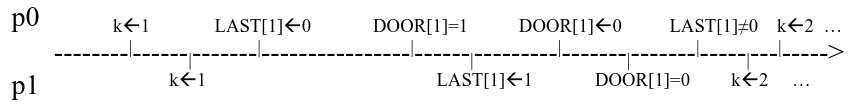
\includegraphics[width=0.8\linewidth]{images/timestamp-generator-blocking.png}
        %\captionof{figure}{Blocking Timestamp Generator temporal sequence.}
    \end{minipage}
   
   For example, if $p_0$ and $p_1$ both enter the loop for $k=1$, $p_0$ might write to \texttt{LAST[1]} and close the door \texttt{DOOR}$\leftarrow$\texttt{0}. Then $p_1$ writes to \texttt{LAST[1]}, causing $p_0$ to fail the \texttt{LAST[k] = i} check and $p_1$ finds the door closed. If they both then move to $k=2$ and repeat this exact timing, they could theoretically loop forever. This lack of progress only occurs during active contention; if one process were to run in isolation, it would successfully secure the next available $k$ and terminate.
    \end{demonstration}
\end{Thm}

\section{Wait-free Stack}
A wait-free implementation of a stack can be constructed using an unbounded array of atomic registers, denoted as \texttt{REG}. In this model, every register in the array is initialized to $\perp$ and supports atomic writes as well as a \texttt{swap(v)} primitive. The swap operation is crucial as it atomically writes a new value into a register and returns the value that was previously stored there. To manage the current position of the stack, a shared atomic register called \texttt{NEXT} is used, which is initialized to 1 and supports fetch\&add operations.

The operations are defined as follows:
\begin{itemize}
    \item \texttt{push(v)}: A process first calls \texttt{NEXT.fetch\&add(1)} to reserve a unique index $i$ in the \texttt{REG} array. It then writes the value $v$ into \texttt{REG[i]}. Because fetch\&add is atomic, every push operation is guaranteed a unique slot, ensuring that no two processes overwrite each other’s data before it can be processed.

\begin{minipage}{\textwidth}
\begin{lstlisting}[mathescape]
push(v) :=
    i $\leftarrow$ NEXT.fetch&add(1)
    REG[i] $\leftarrow$ v
\end{lstlisting}
\captionof{lstlisting}{Wait-free Stack \texttt{push} operation.}
\end{minipage}\\

    \item \texttt{pop()}: A process begins by reading the current value of \texttt{NEXT} and setting \texttt{k=NEXT-1}. It then iterates downwards from $k$ to 1, attempting to "claim" a value by performing \texttt{REG[i].swap(}$\perp$\texttt{)}. If the swap returns a value other than $\perp$, that value is returned as the popped element. If the loop completes without finding a value, it returns $\perp$, indicating the stack is effectively empty.

\begin{minipage}{\textwidth}
\begin{lstlisting}[mathescape]
pop() :=
    k $\leftarrow$ NEXT-1
    for i=k downto 1
        tmp $\leftarrow$ REG[i].swap($\perp$)
        if tmp$\neq$ $\perp$ then return tmp
    return $\perp$
\end{lstlisting}
\captionof{lstlisting}{Wait-free Stack \texttt{pop} operation.}
\end{minipage}\\

\end{itemize}

A significant advantage of this implementation is that process crashes do not compromise the progress of the system. Since the operations are wait-free, every invocation eventually terminates regardless of the behavior of other processes. However, this specific design relies on the unboundedness of the REG array, which is not a realistic assumption for physical hardware.

\section{Non-blocking Bounded Stack}
To address the limitations of unbounded memory, we can implement a \textit{bounded stack}\index{bounded stack} that satisfies the non-blocking progress condition. The core idea behind this implementation is "helping": every operation started by an invoking process is finalized either by that process or by the subsequent process that enters the system.

This implementation utilizes an array \texttt{STACK[0..k]} and a \texttt{TOP} register, both of which support compare\&set (CAS) operations. However, using CAS introduces the \textit{ABA problem}\index{ABA problem}. This occurs when a process reads a value $A$, and before it can perform a CAS to change $A$ to $C$, other processes change the value from $A$ to $B$ and then back to $A$. The CAS would succeed, potentially ignoring the intermediate state change.

To solve this, we use versioning or sequence numbers. In this bounded stack:
\begin{itemize}
    \item Each entry in \texttt{STACK[i]} is a pair $\langle val,seq\_numb\rangle$, initialized to $\langle \perp,0\rangle$. Any modification to a stack slot must increment its sequence number.

    The \texttt{TOP} register is a triple $\langle index,val,seq\_numb\rangle$, initialized to $\langle 0,\perp,1\rangle$. Here, $index$ represents the current top of the stack, $val$ is the value to be placed there, and $seq\_numb$ ensures that every update to the top of the stack is unique.
\end{itemize}

The implementation relies on three primary functions:
\begin{itemize}
    \item \texttt{conclude(i, v, s)} is designed to ensure that the value associated with a stack index is properly written into the \texttt{STACK} array. It reads the current value at \texttt{STACK[i]} and attempts to compare\&set it to the intended value $v$ while incrementing the sequence number to $s$. This ensures that even if a process crashes immediately after updating \texttt{TOP}, the next process to access the stack will finish the work.

\begin{minipage}{\textwidth}
\begin{lstlisting}[mathescape]
conclude(i,v,s) :=
    tmp $\leftarrow$ STACK[i].val
    STACK[i].compare&set($\langle$tmp,s-1$\rangle$,$\langle$v,s$\rangle$)
\end{lstlisting}
\captionof{lstlisting}{Non-blocking Bounded Stack \texttt{conclude} operation.}
\end{minipage}\\
    
    \item \texttt{push(w)}: The process enters a loop where it reads the \texttt{TOP} triple. It first calls conclude to ensure any previous operation is finished. If the index $i$ has reached the limit $k$, it returns \texttt{FULL}. Otherwise, it calculates a \texttt{newtop} containing the incremented index and the new value $w$. It then attempts a \texttt{TOP.compare\&set}. If it succeeds, the push is logically complete.

\begin{minipage}{\textwidth}
\begin{lstlisting}[mathescape]
push(w) :=
    while true do
        $\langle$i,v,s$\rangle$ $\leftarrow$ TOP
        conclude(i,v,s)
        if i=k then return FULL
        newtop $\leftarrow$ $\langle$i+1,w,STACK[i+1].seq_num+1$\rangle$
        if TOP.compare&set($\langle$i,v,s$\rangle$,newtop)
        then return OK
\end{lstlisting}
\captionof{lstlisting}{Non-blocking Bounded Stack \texttt{push} operation.}
\end{minipage}\\
    
    \item \texttt{pop()}: Similar to push, the process reads \texttt{TOP} and calls conclude. If the index is 0, it returns \texttt{EMPTY}. It then attempts to move \texttt{TOP} to the previous index ($i-1$) using compare\&set. If successful, it returns the value $v$ that was at the top.

\begin{minipage}{\textwidth}
\begin{lstlisting}[mathescape]
pop() :=
    while true do
        $\langle$i,v,s$\rangle$ $\leftarrow$ TOP
        conclude(i,v,s)
        if i=0 then return EMPTY
        newtop $\leftarrow$ $\langle$i-1,STACK[i-1]$\rangle$
        if TOP.compare&set($\langle$i,v,s$\rangle$,newtop)
        then return v
\end{lstlisting}
\captionof{lstlisting}{Non-blocking Bounded Stack \texttt{pop} operation.}
\end{minipage}\\
\end{itemize}

\begin{Thm}{Liveness proof in Non-blocking Bounded Stack}{}
    The liveness of this implementation is guaranteed to be non-blocking. 

    \begin{demonstration}
    If a process $p$ fails to complete its compare\&set on \texttt{TOP}, it is because the value of \texttt{TOP} has changed in the interim. Since the only instruction that modifies \texttt{TOP} is the final compare\&set of a successful push or pop, a failure by $p$ implies that at least one other operation has successfully terminated. This satisfies the non-blocking requirement that the system as a whole makes progress.

    The use of the \texttt{conclude} function is vital for correctness during crash failures. In a naive implementation, if a process crashed after updating \texttt{TOP} but before writing the value into the actual stack array, the stack would be left in an inconsistent state. By making the "conclusion" of an operation a shared responsibility—performed both at the end of the current invocation and at the start of the next—the system ensures that the data is always consistently applied before the stack is modified again.
    \end{demonstration}
\end{Thm}

\section{Enhancing Liveness Properties}
In mutual exclusion (MUTEX)-based concurrency, it is a known principle that weak liveness properties, such as deadlock-freedom, can be elevated to stronger ones like bounded bypass. The goal is to apply a similar logic to mutex-free concurrency. Mutex-freedom is defined by the absence of critical sections or locks in the implementation of a concurrent object, ensuring that no process is blocked because another process has paused or crashed while holding a resource.

To achieve stronger liveness in this framework, we introduce the concept of a \textit{Contention Manager}\index{contention manager}. This is a specialized object designed to provide "contention-free periods" or "favorable circumstances" that allow a process to complete its operation without being repeatedly interrupted by others. A contention manager typically provides two primary operations:
\begin{itemize}
    \item \texttt{need\_help(i)}: Invoked by process $p_i$ when it detects contention (e.g., its operation has failed to progress after multiple attempts).
    \item \texttt{stop\_help(i)}: Invoked by $p_i$ once it has successfully completed its operation.
\end{itemize}

This enrichment differs from traditional lock/unlock mechanisms because it must account for fail-stop failures. In a mutex-free system, a process can crash during a contention-free period. Because an asynchronous system cannot inherently distinguish between a crashed process and one that is simply experiencing a long delay, we must rely on \textit{failure detectors}\index{failure detector}. These modules provide processes with (potentially unreliable) information about which other processes in the system have failed, and they are categorized by the quality and accuracy of the information they provide.

\subsection{From obstruction-freedom to non-blocking}
Obstruction-freedom is a weak progress condition where a process is guaranteed to finish its operation only if it eventually executes in isolation for a sufficient amount of time. To "boost" this to a non-blocking property—where at least one process is always guaranteed to make progress—we use a failure detector called \textit{Eventually Restricted Leadership}\index{eventually restricted leadership} ($\Omega_X$).

Given a set of process IDs $X$, the $\Omega_X$ detector provides each process with a local variable, \texttt{ev\_leader(X)}, which satisfies two properties:
\begin{itemize}
    \item \textit{Validity:} The variable always contains a valid process ID from the set.
    \item \textit{Eventual Leadership:} Eventually, all non-crashed processes in $X$ will permanently agree on the same leader, who must itself be a non-crashed process.
\end{itemize}
    
The implementation of this contention manager uses an array of Single-Writer Multiple-Reader (SWMR) atomic registers, \texttt{NEED\_HELP[1..n]}, initialized to \texttt{false}. 

\begin{minipage}{\textwidth}
\begin{lstlisting}[mathescape]
NEED_HELP[1..n] : SWMR atomic R/W boolean registers init at false
\end{lstlisting}
\begin{minipage}{0.45\textwidth}
\begin{lstlisting}[mathescape]
need_help(i) :=
    NEED_HELP[i] $\leftarrow$ true
    repeat
        X $\leftarrow$ {j : NEED_HELP[j]}
    until ev_leader(X) = i
\end{lstlisting}
\end{minipage}
\hfill
\begin{minipage}{0.45\textwidth}
\begin{lstlisting}[mathescape]
stop_help(i) :=
    NEED_HELP[i] $\leftarrow$ false



\end{lstlisting}
\end{minipage}
\captionof{lstlisting}{From obstruction-freedom to non-blocking.}
\end{minipage}\\

When a process $p_i$ calls \texttt{need\_help(i)}, it sets its register to true and then enters a loop. Inside this loop, it identifies the set $X$ of all processes currently requesting help and waits until the failure detector $\Omega_X$ designates $p_i$ as the leader. Once $p_i$ finishes its task, it calls \texttt{stop\_help(i)} to set its register back to \texttt{false}.

\begin{Thm}{From obstruction-freedom to non-blocking}{}
    The contention manager described above successfully transforms an obstruction-free implementation into a non-blocking one. 
\begin{demonstration}
    This is proven by contradiction: assume there is a time $\tau$ after which several concurrent operations never terminate. Let $Q$ be the set of processes attempting these operations.
    \begin{itemize}
        \item Due to the enrichment, eventually all processes in $Q$ will set their \texttt{NEED\_HELP} flags to \texttt{true} forever.
        \item Crashed processes outside of $Q$ will eventually stop modifying their flags.
        \item This leads to a point where all processes in $Q$ compute the same set $X$ of processes needing help.
        \item By the definition of $\Omega_X$, a single leader will eventually be elected from $X$ (and since the leader must be non-crashed, it must be in $Q$).
        \item This leader will then be the only process allowed to proceed, effectively running in isolation. Because the underlying implementation is obstruction-free, the leader is guaranteed to terminate, contradicting the assumption that no process in Q makes progress.
    \end{itemize}
\end{demonstration}
\end{Thm}

Implementing $\Omega$ is impossible in a purely asynchronous system because crashes are indistinguishable from long delays. Therefore, we must introduce timing constraints. One common approach assumes:
\begin{enumerate}
    \item \textit{Bounded Write Delay:} There exists a correct process $p_L$ and a time interval $\Delta$ such that $p_L$ writes to its progress register at least once every $\Delta$ time units.
    \item \textit{Timer Accuracy:} There are enough correct processes with timers that will eventually not expire "too early," allowing them to correctly identify the progress of $p_L$.
\end{enumerate}

The implementation idea involves a \texttt{PROGRESS[1..n]} array where each process regularly increments its entry to signal it is alive. If process $p_i$ does not see progress from $p_j$ within a certain (guessed) time interval, it "suspects" $p_j$. The leader is then chosen as the "least suspected" process. To handle the uncertainty of the system's speed, processes dynamically adjust their suspicion timers by tracking the number of times they have suspected others (\texttt{SUSPECT[i, j]}) and summing these values to guess a duration that eventually exceeds the actual system delay $\Delta$.

\subsection{From obstruction-freedom to wait-freedom}
To achieve wait-freedom—where every correct process is guaranteed to finish its operation in a finite number of steps—a stronger failure detector is required: the \textit{Eventually Perfect Failure Detector}\index{eventually perfect failure detector} ($\diamondsuit P$). $\diamondsuit P$ provides:
\begin{itemize}
    \item \textit{Eventual Completeness:} Eventually, every crashed process is suspected by every correct process.
    \item \textit{Eventual Accuracy:} Eventually, no correct process is suspected by any correct process.

\end{itemize}

In the hierarchy of failure detectors, $\diamondsuit P$ is strictly stronger than $\Omega_X$. We can build $\Omega_X$ from $\diamondsuit P$ by having each process pick the process with the minimum ID among those not currently suspected. However, $\Omega_X$ cannot build $\diamondsuit P$ because $\Omega_X$ only guarantees one common leader, while $\diamondsuit P$ requires eventual perfect knowledge of all crashes.

The wait-free manager utilizes a weak timestamp generator, which ensures that for any timestamp $t$ returned, only a finite number of subsequent requests can receive a timestamp smaller than or equal to $t$. The algorithm works as follows:

\begin{minipage}{\textwidth}
\begin{lstlisting}[mathescape]
TS[1..n] : SWMR atomic R/W registers init at 0
\end{lstlisting}
\begin{lstlisting}[mathescape]
need_help(i) :=
    TS[i] $\leftarrow$ weak_ts()
    repeat
        competing $\leftarrow$ {j : TS[j]$\neq$0 $\land$ j $\notin$ suspected$_i$}
        $\langle$t,j$\rangle$ $\leftarrow$ min{$\langle$TS[x],x$\rangle$ | x $\in$ competing}
    until j = i
\end{lstlisting}
\begin{lstlisting}[mathescape]
stop_help(i) :=
    TS[i] $\leftarrow$ 0 
\end{lstlisting}
\captionof{lstlisting}{From obstruction-freedom to wait-freedom.}
\end{minipage}

\begin{itemize}
    \item \texttt{need\_help(i)}: Process $p_i$ obtains a timestamp \texttt{TS[i]}. It then loops, identifying a set of "competing" processes (those with non-zero timestamps who are not currently suspected by the failure detector). It waits until its own timestamp-identity pair $\langle TS[i],i\rangle$ is the minimum among all competitors.
    \item \texttt{stop\_help(i)}: Once the operation is done, $p_i$ resets \texttt{TS[i]} to 0.
\end{itemize}

\begin{Thm}{Wait-freedom proof of from obstruction-freedom to wait-freedom}{}
\begin{demonstration}
    Suppose a correct process $p_i$ never terminates its invocation. Let its timestamp be $t_i$, and assume $\langle t_i,i\rangle$ is the minimum such pair that fails to terminate.
    \begin{itemize}
        \item Any process that crashes will eventually be suspected by $p_i$ (due to $\diamondsuit P$ completeness) and will be removed from the competing set.
        \item Any process with a smaller timestamp than $p_i$ must either crash or terminate (since $p_i$ is the minimum non-terminating case).
        \item Once these finite "older" invocations are cleared and crashed processes are suspected, $p_i$ will eventually have the minimum timestamp and be allowed to run in isolation.
        \item Because the implementation is obstruction-free, $p_i$ will eventually finish.
    \end{itemize}
    
    To implement $\diamondsuit P$ itself, the system relies on processes having an eventual upper bound on write delays. By adjusting timers based on whether a process's suspicion was correct or "premature," the system eventually reaches a state where only actually crashed processes are suspected.
\end{demonstration}
\end{Thm}

\chapter{Universal Object}
In the study of concurrent systems, a fundamental question arises regarding the implementation of complex objects: given objects of a specific type $T$ and a basic object type $Z$, is it possible to create a wait-free implementation of $Z$ using only objects of type $T$ and atomic Read/Write (R/W) registers? This question addresses the relative "synchronization power" of different object types.

To answer this, we must first define what constitutes a "type." An object type is defined by two primary components:
\begin{enumerate}
    \item \textit{The State Space:} The set of all possible values that an object of that type can hold.
    \item \textit{The Operations:} A set of operations used to manipulate the object, each accompanied by a sequential specification. This specification describes the conditions for invocation and the resulting effect on the object’s state.
\end{enumerate}
    
In this context, we focus on types with operations that are \textit{total}\index{total operation} and \textit{sequentially specified}\index{sequentially specified operation}. An operation is "total" if it can be invoked regardless of the current state of the object. A sequential specification implies that the object’s behavior is entirely determined by the sequence of operations performed on it. Formally, this is represented by a transition function $\delta(s,op(args))=\{\langle s_1,res_1\rangle,\ldots,\langle s_k,res_k\rangle\}$. In a \textit{deterministic object}\index{deterministic object}, $k=1$, meaning for every state and operation, there is exactly one resulting state and one output.

An object type $T_U$ is considered \textit{universal}\index{universal object type} if it is powerful enough to implement any other object type in a wait-free manner, using only $T_U$ and atomic R/W registers.

\section{Consensus Object}
A \textit{consensus object}\index{consensus object} is a "one-shot" object—meaning each process can access it only once. It provides a single operation, \texttt{propose(v)}, which must satisfy four critical properties:
\begin{itemize}
    \item \textit{Validity:} The value decided upon must have been proposed by at least one participant.
    \item \textit{Integrity:} Each process can decide on a value at most once.
    \item \textit{Agreement:} All processes that decide must decide on the same value.
    \item \textit{Wait-freedom:} Any correct process that invokes the operation will eventually terminate.
\end{itemize}

\begin{minipage}{\textwidth}
\begin{lstlisting}[mathescape]
propose(v) := if X = $\perp$ then X $\leftarrow$ v
              return X
\end{lstlisting}
\captionof{lstlisting}{Consensus object implementation.}
\end{minipage}\\
    
Conceptually, one could think of implementing a consensus object using a register $X$ initialized to a null value ($\perp$). The \texttt{propose(v)} operation would atomically check if $X$ is $\perp$; if so, it writes $v$ to $X$. Regardless of whether the write occurred, the operation returns the value currently in $X$. This "winner-takes-all" logic ensures that the first value written becomes the permanent decision.

The core thesis of the universality of consensus is that if we have consensus objects, we can implement any other object $O$ of type $Z$. This is achieved by having every participant run a local copy of $O$, all starting at the same initial state. By using consensus objects to create a total order of operations, processes can "force" their local simulations to follow the exact same sequence. Because the objects are deterministic, consistent local copies result in a consistent global state.

To understand the wait-free implementation, we first look at a simpler, non-blocking (but not wait-free) construction for deterministic objects.

\begin{minipage}{\textwidth}
\begin{lstlisting}[mathescape]
result$_i$ $\leftarrow$ $\perp$
invoc$_i$ $\leftarrow$ $\langle$op(args), i$\rangle$
wait result$_i$ $\neq$ $\perp$
return result$_i$
\end{lstlisting}
\captionof{lstlisting}{\texttt{op(arg)} by $p_i$ on $Z$ for non-blocking, not wait-free deterministic objects.}
\end{minipage}\\

In this model, a process $p_i$ wanting to execute an operation \texttt{op(args)} on an object $Z$ uses two local variables: \texttt{result}$_i$ (to store the final output) and \texttt{invoc}$_i$ (to store the operation and the process ID).

The system uses an unbounded array of consensus objects, \texttt{CONS}. 

\begin{minipage}{\textwidth}
\begin{lstlisting}[mathescape]
k $\leftarrow$ 0
z$_i$ $\leftarrow$ Z.init()
while true
    if invoc$_i$ $\neq$ $\perp$ then
        k++
        exec$_i$ $\leftarrow$ CONS[k].propose(invoc$_i$)
        $\langle$z$_i$, res$\rangle$ $\leftarrow$ $\delta$(z$_i$, $\pi_1$(exec$_i$))
        if $\pi_2$(exec$_i$) = i then
            invoc$_i$ $\leftarrow$ $\perp$
            result$_i$ $\leftarrow$ res
\end{lstlisting}
\captionof{lstlisting}{Local simulation of $Z$ by $p_i$ for non-blocking, non wait-free deterministic objects.}
\end{minipage}\\

Each process runs a simulation of $Z$ in a local variable $z_i$. The logic proceeds in a loop:
\begin{itemize}
    \item Process $p_i$ increments a counter $k$ to move to the next consensus instance.
    \item It proposes its operation \texttt{invoc}$_i$ to \texttt{CONS[k]}.
    \item The consensus object returns a winning operation, \texttt{exec}$_i$. This may be $p_i$'s operation or an operation proposed by another process.
    \item Process $p_i$ applies \texttt{exec}$_i$ to its local state $z_i$ using the transition function $\delta$.
    \item If the operation that won the consensus was indeed $p_i$'s operation $(\pi_2(exec_i)=i), p_i$ updates its \texttt{result}$_i$ and clears its pending invocation.
\end{itemize}

While this ensures that all processes see the same operations in the same order, it is not wait-free. A process could potentially be "starved" if it consistently loses the consensus to other processes, preventing its operation from ever being executed.

To achieve wait-freedom, the construction must ensure that every process's operation is eventually executed, even if the process itself does not "win" the consensus. This is handled through a "helping" mechanism.

The shared state involves an array of Single-Writer/Multi-Reader (SWMR) atomic registers called \texttt{LAST\_OP[1..n]}. Each register $i$ stores a pair: the operation $p_i$ wants to perform and a sequence number. Locally, each process $p_j$ maintains an array \texttt{last\_sn\_j[1..n]} to track which operations from other processes it has already executed.

\begin{minipage}{\textwidth}
\begin{lstlisting}[mathescape]
result$_i$ $\leftarrow$ $\perp$
LAST_OP[i] $\leftarrow$ $\langle$op(args),
             last_sn$_i$[i]+1$\rangle$
wait result$_i$ $\neq$ $\perp$
return result$_i$
\end{lstlisting}
\captionof{lstlisting}{\texttt{op(arg)} by $p_i$ on $Z$ for non-blocking, wait-free deterministic objects.}
\end{minipage}\\

\begin{minipage}{\textwidth}
\begin{lstlisting}[mathescape]
k $\leftarrow$ 0
z$_i$ $\leftarrow$ Z.init()
while true
    invoc$_i$ $\leftarrow$ $\epsilon$
    $\forall$ j = 1..n
        if $\pi_2$(LAST_OP[j])>last_sn$_i$[j]
        then invoc$_i$.append(
                $\langle$$\pi_1$(LAST_OP[j]),j$\rangle$ )
    if invoc$_i$ $\neq$ $\epsilon$ then
        k++
        exec$_i$ $\leftarrow$ CONS[k].propose(invoc$_i$)
        for r=1 to |exec$_i$|
            $\langle$z$_i$,res$\rangle$ $\leftarrow$ $\delta$(z$_i$,$\pi_1$(exec$_i$[r]))
            j $\leftarrow$ $\pi_2$(exec$_i$[r])
            last_sn$_i$[j]++
            if i=j then result$_i$ $\leftarrow$ res
\end{lstlisting}
\captionof{lstlisting}{Local simulation of $Z$ by $p_i$ for non-blocking, wait-free deterministic objects.}
\end{minipage}\\

In this construction, the simulation loop is more complex. When a process $p_i$ wants to perform an operation, it first announces it by writing to \texttt{LAST\_OP[i]} with an incremented sequence number. It then enters the simulation loop. Instead of proposing a single operation to the consensus object, it proposes a list of all pending operations it sees in the \texttt{LAST\_OP} array (those where the sequence number in the register is greater than the one it has locally recorded).

The consensus object \texttt{CONS[k]} now decides on a list of operations. When $p_i$ receives the winning list \texttt{exec}$_i$, it iterates through the entire list, applying each operation to its local state $z_i$ and updating the corresponding sequence numbers in \texttt{last\_sn\_i}. If $p_i$ finds its own operation within the list, it can finally return the result.

The correctness of this construction is established through three primary lemmas:

\begin{Lemma}{The construction is wait-free}{}
The construction is wait-free.
\begin{demonstration}
To prove wait-freedom, we must show that $p_i$ eventually finds its operation in a decided list. Because $p_i$ publishes its operation in \texttt{LAST\_OP[i]} with an increased sequence number, any process (including $p_i$ itself) that participates in a subsequent consensus will see this operation and include it in their proposed list. Since at least one correct process will eventually succeed in a consensus round, $p_i$'s operation is guaranteed to be part of an agreed-upon list.  
\end{demonstration}
\end{Lemma}

\begin{Lemma}{All operations are executed exactly once}{}
All operations are executed exactly once.
\begin{demonstration}
We must ensure that an operation isn't applied to the state multiple times. $p_i$ cannot start a new operation until its current one is executed. Furthermore, every process tracks sequence numbers locally (\texttt{last\_sn}). When a process processes a list from consensus, it only appends operations to its "to-be-executed" list if the sequence number is new. If a process $p_j$ participates in consensus $k$, it updates its local sequence numbers before forming a proposal for consensus $k+1$, ensuring it doesn't propose the same operation twice.
\end{demonstration}
\end{Lemma}

\begin{Lemma}{Consistency and Sequential Specification}{}
Consistency and sequential specification.
\begin{demonstration}
Because all processes access the consensus objects in the same order (\texttt{CONS[1]}, \texttt{CONS[2]}, ...) and consensus guarantees all processes receive the same list, every process applies the same sequence of operations to their local copies. Since the starting states were identical and the transitions are deterministic, the local states $z_i$ remain consistent across all processes.
\end{demonstration}
\end{Lemma}

It is important to note that while this construction is wait-free, it does not provide bounded wait-freedom. If a process $p_i$ is suspended for a significant amount of time, it may wake up to find an immense "log" of agreed-upon lists in the \texttt{CONS} array. It must catch up by locally executing all these operations before it can complete its own current operation. This catch-up phase can be arbitrarily long, meaning the time to complete an operation is not strictly bounded.

The previous wait-free constructions assume that the object $Z$ is deterministic, meaning that for any given state and operation, there is exactly one possible resulting state and output. However, many concurrent objects have non-deterministic specifications where the transition function $\delta(s,op(args))$ returns a set of possible pairs $\{\langle s_1,res_1\rangle,\ldots\langle s_k,res_k\rangle\}$. In such cases, if processes simply agree on the order of operations, their local simulations might diverge if they independently pick different outcomes from the set of possibilities.

To maintain consistency across all local copies in a wait-free manner, processes must be forced to choose the same transition for every non-deterministic step. The slides suggest three potential solutions:
\begin{enumerate}
    \item \textit{The "Brute Force" Solution:} This approach involves "canceling" the non-determinism by fixing a rule a priori. For every possible pair of state and operation, one specific outcome from the set $\delta$ is pre-selected as the "correct" one. This effectively turns a non-deterministic object into a deterministic one before the simulation begins.
    \item \textit{Additional Consensus Objects:} A more dynamic approach is to use a new consensus object for every single operation. These additional consensus instances would be used specifically to agree on which outcome ($\langle s_i,res_i\rangle$) to choose from the set of valid transitions returned by $\delta$.
    \item \textit{Reusing the Primary Consensus Object:} Instead of using separate consensus objects for the choice of outcome, the proposals sent to the main consensus array (\texttt{CONS[k]}) can be expanded. A process would not only propose the list of operations to be performed but also pre-calculate and propose the resulting state and return value for each operation in that list. This ensures that when the consensus returns an agreed-upon list, it also includes the agreed-upon results, maintaining local consistency.
\end{enumerate}

\section{From Binary to Multivalued Consensus}
A fundamental question in synchronization is whether the complexity of the data we agree upon matters. \textit{Binary consensus}\index{binary consensus} allows only two possible proposals (typically 0 and 1). \textit{Multivalued consensus}\index{multivalued consensus} allows for an unbounded set of possible values. We can implement a multivalued consensus object using only binary consensus objects and registers.

The construction for \textit{unbounded multivalued consensus} (where the number of possible values is not fixed) uses an array of $n$ binary consensus objects (\texttt{BC[1..n]}) and an array of $n$ proposal registers (\texttt{PROP[1..n]}). 

\begin{figure}[ht]
    \centering
    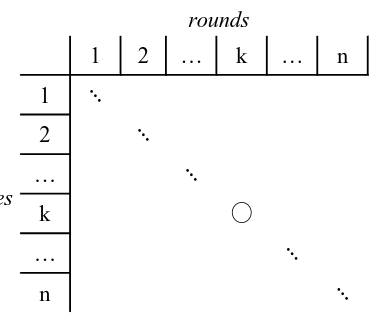
\includegraphics[width=0.3\linewidth]{images/multivalued-consensus.png}
    \caption{Multivalued consensus (with unbounded values).}
    \label{fig:multivalued-consensus}
\end{figure}

\begin{minipage}{\textwidth}
\begin{lstlisting}[mathescape]
PROP[1..n] array of n proposals, all init at $\perp$
BC[1..n] array of n binary consensus objects
\end{lstlisting}
\begin{lstlisting}[mathescape]
mv_propose(i,v) :=
    PROP[i] $\leftarrow$ v
    for k=1 to n do
        if PROP[k] $\neq$ $\perp$ then res $\leftarrow$ BC[k].propose(1)
                        else res $\leftarrow$ BC[k].propose(0)
        if res = 1 then return PROP[k]
    wait forever
\end{lstlisting}
\captionof{lstlisting}{Multivalued consensus (with unbounded values).}
\end{minipage}\\

Each process $p_i$ proposing a value $v$ follows this logic:
\begin{enumerate}
    \item It writes its value $v$ to its specific register \texttt{PROP[i]}.
    \item It then iterates through all processes from $k=1$ to $n$.
    \item For each $k$, it checks if process $p_k$ has written a proposal. If \texttt{PROP[k]} is not empty, it proposes 1 to the binary consensus \texttt{BC[k]}. Otherwise, it proposes 0.
    \item If the binary consensus \texttt{BC[k]} returns 1, it means the system has agreed to use the value proposed by $p_k$. Process $p_i$ then returns \texttt{PROP[k]} as the decided value.
\end{enumerate}

\begin{Demonstration}{Proof of Correcteness for Multivalued Consensus (with unbounded values)}{}
\begin{itemize}
    \item \textit{Validity:} If a process $p_x$ is the first to write a proposal, any process entering the loop later will see \texttt{PROP[x]} is not empty and propose 1 to \texttt{BC[x]}. Thus, at least one binary consensus will eventually return 1.
    \item \textit{Agreement:} Because every process iterates through the binary consensus objects in the same order (1 to $n$), they will all stop at the same first index $y$ where \texttt{BC[y]} returns 1. Consequently, they all decide on the same value \texttt{PROP[y]}.
\end{itemize}
\end{Demonstration}

If the number of possible values $k$ is known and bounded, we can use a more efficient construction. By representing each value as a binary string of length $h=\log_2k$, we can decide the final value one bit at a time.

In this \textit{bounded construction}, we use an array of $h$ binary consensus objects (\texttt{BC[1..h]}). Each process $p_i$ writes its proposal as a bit-string in \texttt{PROP[i]}. 

\begin{minipage}{\textwidth}
\begin{lstlisting}[mathescape]
PROP[1..n][1..h] array of n h-bits proposals, all init at $\perp$
BC[1..h] array of h binary consensus objects
\end{lstlisting}
\begin{lstlisting}[mathescape]
bmv_propose(i,v) :=
    PROP[i] $\leftarrow$ binary_repr$_h$(v)
    for k=1 to h do
        P $\leftarrow$ {PROP[j][k] | PROP[j] $\neq$ $\perp$ $\land$ PROP[j][1..k-1]=res[1..k-1]}
        let b be an element of P
        res[k] $\leftarrow$ BC[k].propose(b)
    return value(res)
\end{lstlisting}
\captionof{lstlisting}{Multivalued consensus (with bounded values).}
\end{minipage}\\

The processes then loop from $k=1$ to $h$ to decide each bit:
\begin{enumerate}
    \item In each round $k$, a process identifies the set $P$ of possible bits. This set contains the $k$-th bits of all proposals currently in the registers that match the prefix already decided in rounds 1 to $k-1$.
    \item The process picks a bit $b$ from this set $P$ and proposes it to \texttt{BC[k]}.
    \item The result of \texttt{BC[k]} becomes the $k$-th bit of the final decided value.
\end{enumerate}

\begin{Demonstration}{Proof of Correctness Analysis for Multivalued consensus (with bounded values)}{}
\begin{itemize}
    \item \textit{Wait-freedom and Integrity:} These are inherited from the underlying binary consensus objects and the fixed number of iterations ($h$).
    \item \textit{Agreement:} This is guaranteed because each bit is decided by a binary consensus object, which ensures all processes see the same bit for each position in the string.
    \item \textit{Validity:} The construction of the set $P$ is vital. By only proposing bits that belong to a proposal matching the existing prefix, the algorithm ensures that the final "assembled" bit-string is not a hybrid of different proposals, but rather matches at least one full proposal that was actually submitted by a participant. For every bit $b\in P$ selected, there is at least one process $p_j$ whose proposal matches the decided bits up to that point. By the time the loop reaches $h$, the final string must equal some $p_j$'s original proposal.
\end{itemize}
\end{Demonstration}

\chapter{Consensus Number}
In the study of concurrent systems, a fundamental question arises: which types of shared objects allow for a wait-free implementation of binary consensus? The answer is not absolute; rather, it depends entirely on the number of participating processes. To categorize the "synchronization power" of different object types, we use the concept of a consensus number.

The \textit{consensus number}\index{consensus number} of an object of type $T$, denoted as $CN(T)$, is defined as the greatest number $n$ such that it is possible to provide a wait-free implementation of a consensus object in a system of $n$ processes using only objects of type $T$ and standard atomic read/write (R/W) registers. For every object type $T$, the consensus number is at least 1, as a single process can always "decide" its own proposal. If there is no upper bound on the number of processes for which a wait-free implementation exists, we say $CN(T)=\infty$.

This definition leads to a powerful hierarchy theorem.

\begin{Thm}{Consensus Number}{}
If $CN(T_1)<CN(T_2)$, then there is no wait-free implementation of objects of type $T_2$ in a system of $n$ processes that uses only objects of type $T_1$ and atomic R/W registers, provided that $CN(T_1)<n\leq CN(T_2)$. This theorem establishes that object types with higher consensus numbers are strictly more powerful than those with lower ones.
\begin{demonstration}
The proof of this hierarchy relies on contradiction. If we assume such an implementation exists, then because $n\leq CN(T_2)$, we know consensus can be implemented using $T_2$. By substituting the $T_1$-based implementation for $T_2$, we would effectively have a wait-free consensus for $n$ processes using only $T_1$. However, this contradicts the definition of $CN(T_1)$, which states that $T_1$ cannot solve consensus for any number of processes greater than $CN(T_1)$.
\end{demonstration}
\end{Thm}

\section{Schedules and Configurations}
To formally prove the limits of consensus, we must define the state of the system. A \textit{Schedule}\index{schedule} ($S$) is a sequence of operation invocations issued by processes. A \textit{Configuration}\index{configuration} ($C$) represents the global state of the system at any given time, encompassing the values of all shared memory objects and the local state of every process. If we apply a schedule $S$ starting from configuration $C$, the resulting state is denoted as $S(C)$.

When analyzing a binary consensus algorithm $A$, we categorize configurations based on their potential outcomes:
\begin{itemize}
    \item  \textit{v-valent:}\index{v-valent} A configuration is v-valent (where $v\in \{0,1\}$) if every possible execution starting from that configuration eventually decides the value $v$.
    \item \textit{Monovalent:}\index{monovalent} A configuration that is either 0-valent or 1-valent.
    \item \textit{Bivalent:}\index{bivalent} A configuration that is not monovalent, meaning that both a decision of 0 and a decision of 1 are still possible depending on the subsequent scheduling of processes.
\end{itemize}

\begin{Thm}{Fundamental theorem}{}
A critical result in distributed computing is that if an algorithm $A$ wait-free implements binary consensus for $n$ processes, there must exist an initial configuration that is bivalent.
\begin{demonstration}
We can prove this by considering a sequence of initial configurations $C_0$,$C_1$,$\ldots$,$C_n$, where $C_i$ is the configuration where processes $p_1$ through $p_i$ propose 1, and the remaining processes propose 0. By the validity requirement of consensus, $C_0$ must be 0-valent (all propose 0) and $C_n$ must be 1-valent (all propose 1).

If we assume for contradiction that all initial configurations are monovalent, there must be some index $i$ where $C_{i-1}$ is 0-valent and $C_i$ is 1-valent. These two configurations differ only in the proposal of process $p_i$. Now, consider a schedule $S$ where $p_i$ is "asleep" or blocked for a long period. By the wait-freedom property, the other processes must eventually decide even without $p_i$. In $C_{i-1}$, they must decide 0. Because $p_i$ is sleeping, the other processes cannot distinguish between $C_{i-1}$ and $C_i$, so they must also decide 0 in $C_i$. This leads to a contradiction: if $p_i$ wakes up in $C_i$ and decides 1 (to satisfy its own valence), it violates agreement; if it decides 0, it contradicts the 1-valence of $C_i$. Thus, an initial bivalent state must exist.
\end{demonstration}
\end{Thm}

\begin{Thm}{CN(Atomic R/W registers) = 1}{}
Atomic read/write registers are the most basic shared memory objects, and it can be proven that they cannot solve consensus for even two processes ($n=2$).
\begin{demonstration}
To prove \textit{CN(Atomic R/W)=1} by contradiction, we assume an algorithm $A$ exists for two processes, $p$ and $q$. We start from a bivalent initial configuration $C$ and follow a schedule $S$ until we reach a "maximally bivalent" configuration $C'$. In $C'$, any move by $p$ leads to a 0-valent state, and any move by $q$ leads to a 1-valent state. We then analyze the possible operations $p$ and $q$ could perform on registers $R_1$ and $R_2$:
\begin{enumerate}
    \item $R_1\neq R_2$: If they access different registers, their operations commute. The state $q(p(C'))$ would be the same as $p(q(C'))$. However, $q(p(C'))$ must be 0-valent (since $p(C')$ was 0-valent) and $p(q(C'))$ must be 1-valent (since $q(C')$ was 1-valent). This is a contradiction.
    \item $R_1=R_2$ and both read: Reading does not change the shared state. Thus, the global state after both read is the same regardless of order, leading to the same contradiction as case 1.
    \item $R_1=R_2$, one reads and one writes: Suppose $p$ reads and $q$ writes. Only $p$ can see the result of its read (it's a local state change). If we let $q$ run until it decides while $p$ is stopped, $q$ will decide 1 because $q(C')$ is 1-valent. If we then look at the configuration $p(C')$ and let $q$ run the same schedule, $q$ cannot distinguish $p(C')$ from $C'$ because the shared register looks the same. $q$ will decide 1 again. If we then reactivate $p$, no matter what it decides, it either violates agreement or its own 0-valence.
    \item $R_1=R_2$ and both write: If $q$ writes after $p$, the value written by $p$ is overwritten and lost. Therefore, $q(p(C'))$ is indistinguishable from $q(C')$ for process $q$. This leads to the same contradiction as case 3.
\end{enumerate}

Because all cases lead to a contradiction, atomic R/W registers cannot solve consensus for 2 processes.
\end{demonstration}
\end{Thm}

The test\&set (T\&S) operation is more powerful. A T\&S object maintains a value (initially 0). The operation \texttt{test\&set()} atomically sets the value to 1 and returns the old value. We can implement 2-process consensus using T\&S as follows:
Each process $i\in\{0,1\}$ writes its proposal to a shared array \texttt{PROP[i]}. Then, it calls \texttt{TS.test\&set()}. If the returned value is 0, the process knows it was the first to arrive and returns its own proposal. If the returned value is 1, it returns the proposal of the other process ($1-i$). This satisfies validity, wait-freedom, and agreement.

\begin{minipage}{\textwidth}
\begin{lstlisting}[mathescape]
TS a test&set object init at 0
PROP array of proposals, init at whatever
\end{lstlisting}
\begin{lstlisting}[mathescape]
propose(i, v) :=
    PROP[i] $\leftarrow$ v
    if TS.test&set() = 0 then return PROP[i] else return PROP[1-i]
\end{lstlisting}
\captionof{lstlisting}{CN(Test\&set) = 2.}
\end{minipage}\\

\begin{Thm}{CN(Test\&set) $\neq$ 3}{}
However, test\&set cannot solve consensus for 3 processes. 
\begin{demonstration}
The proof structure is similar to the R/W proof: we find a maximally bivalent configuration $C'$ for three processes ($p,q,r$). If $p$ and $q$ both attempt to perform a test\&set on the same object, the global state results in the object being set to 1. The only difference between $p(q(C'))$ and $q(p(C'))$ is the local register of $p$ and $q$ (who saw the 0 and who saw the 1). If we stop $p$ and $q$ and let $r$ run, $r$ cannot distinguish between these two states and must decide the same value in both, leading to a contradiction of the valences of $p(C')$ and $q(C')$.
\end{demonstration}
\end{Thm}

Other common synchronization primitives also fall into specific tiers of the hierarchy:
\begin{itemize}
    \item \textit{Swap and Fetch\&Add (CN=2):} Like test\&set, these can solve 2-process consensus by having the first process to "win" the operation return its own value and the second return the other's. For swap, a process swaps its ID into a register; if it receives the initial $\perp$, it wins. For fetch\&add, the process that receives the initial 0 wins.

\begin{minipage}{\textwidth}
\begin{lstlisting}[mathescape]
S a swap object init at $\perp$
PROP array of proposals, init at whatever
\end{lstlisting}
\begin{lstlisting}[mathescape]
propose(i, v) :=
    PROP[i] $\leftarrow$ v
    if S.swap(i) = $\perp$ then return PROP[i] else return PROP[1-i]
\end{lstlisting}
\begin{lstlisting}[mathescape]
FA a fetch&add object init at 0
PROP array of proposals, init at whatever
\end{lstlisting}
\begin{lstlisting}[mathescape]
propose(i, v) :=
    PROP[i] $\leftarrow$ v
    if FA.fetch&add(1) = 0 then return PROP[i] else return PROP[1-i]
\end{lstlisting}
\captionof{lstlisting}{CN(Swap) = CN(Fetch\&add) = 2.}
\end{minipage}\\
    
    \item \textit{Compare\&Swap (CN=$\infty$):} The compare\&swap(old, new) operation is universal. It checks if the current value matches old; if so, it updates it to new and returns the actual previous value.

\begin{minipage}{\textwidth}
\begin{lstlisting}[mathescape]
X.compare&swap(old,new) :=
    tmp $\leftarrow$ X
    if tmp = old then X $\leftarrow$ new
    return tmp
\end{lstlisting}
\begin{lstlisting}[mathescape]
CS a compare&swap object init at $\perp$
\end{lstlisting}
\begin{lstlisting}[mathescape]
propose(v) :=
    tmp $\leftarrow$ CS.compare&swap($\perp$,v)
    if tmp = $\perp$ then return v else return tmp
\end{lstlisting}
\captionof{lstlisting}{CN(Swap) = CN(Fetch\&add) = 2.}
\end{minipage}\\
    
\end{itemize}
    
To implement consensus for any number of processes using compare\&swap, we initialize a CS object to $\perp$. Every process calls \texttt{CS.compare\&swap($\perp$, v)}. The very first process to execute this will successfully change $\perp$ to its proposal $v$ and receive $\perp$ back, thus deciding $v$. Every subsequent process will find that the value is no longer $\perp$, the swap will fail, and they will receive the value $v$ proposed by the first process. Since they all receive and return the same $v$, consensus is achieved for any $n$.